% =============================================================================
%  Project report — 062047 Numerical Optimization for Control
%  Rolling-horizon A* + nonlinear MPC for map-free navigation (Go2_navigation)
%
%  Built on the PoliMi article-format template (see Thesis.tex, left untouched).
%  Compile with:  pdflatex Report && bibtex Report && pdflatex Report x2
% =============================================================================

\documentclass[11pt,a4paper]{article}

%------------------------------------------------------------------------------
%	REQUIRED PACKAGES AND  CONFIGURATIONS
%------------------------------------------------------------------------------
% PACKAGES FOR TITLES
\usepackage{titlesec}
\usepackage{color}

% PACKAGES FOR LANGUAGE AND FONT
\usepackage[utf8]{inputenc}
\usepackage[english]{babel}
\usepackage[T1]{fontenc}

% PACKAGES FOR IMAGES
\usepackage{graphicx}
\graphicspath{{Images/}}
\usepackage{eso-pic}
\usepackage{subfig}
\usepackage{caption}
\usepackage{transparent}

% PACKAGES FOR VECTOR DIAGRAMS
\usepackage{tikz}
\usetikzlibrary{arrows.meta,positioning,fit,calc,backgrounds}

% STANDARD MATH PACKAGES
\usepackage{amsmath}
\usepackage{amssymb}
\usepackage{amsthm}
\usepackage{bm}
\usepackage[overload]{empheq}

% PACKAGES FOR TABLES
\usepackage{tabularx}
\usepackage{booktabs}
\usepackage{multirow}
\usepackage{longtable}
\usepackage{colortbl}

% PACKAGES FOR ALGORITHMS (PSEUDO-CODE)
\usepackage{algorithm}
\usepackage{algorithmic}

% PACKAGES FOR REFERENCES & BIBLIOGRAPHY
\usepackage[colorlinks=true,linkcolor=black,anchorcolor=black,citecolor=black,filecolor=black,menucolor=black,runcolor=black,urlcolor=black]{hyperref}
\usepackage{cleveref}
\usepackage[square, numbers, sort&compress]{natbib}
\bibliographystyle{plain}

% PACKAGES FOR THE APPENDIX
\usepackage{appendix}

% PACKAGES FOR ITEMIZE & ENUMERATES
\usepackage{enumitem}

% OTHER PACKAGES
\usepackage{amsthm,thmtools,xcolor}
\usepackage{comment}
\usepackage{fancyhdr}
\usepackage{tcolorbox}

%-------------------------------------------------------------------------
%	NEW COMMANDS DEFINED
%-------------------------------------------------------------------------
\newcommand{\bea}{\begin{eqnarray}}
\newcommand{\eea}{\end{eqnarray}}
\newcommand{\e}[1]{\times 10^{#1}}
\newcommand{\pdev}[2]{\frac{\partial#1}{\partial#2}}

% Problem-specific shorthands
\newcommand{\R}{\mathbb{R}}
\newcommand{\astar}{$A^\star$}
\newcommand{\Astar}{A^\star}
\newcommand{\Jobs}{J_{\mathrm{obs}}}
\newcommand{\Wobs}{W_{\mathrm{obs}}}
\newcommand{\aobs}{\alpha_{\mathrm{obs}}}
\newcommand{\robs}{r_{\mathrm{obs}}}
\newcommand{\Rjerk}{R_{\mathrm{jerk}}}
\newcommand{\thn}{\theta_0}
\newcommand{\thst}{\theta_{\mathrm{dep}}}
\newcommand{\Tstr}{T_{\mathrm{str}}}
\newcommand{\Tst}{T_{\mathrm{st}}}
\newcommand{\Tsw}{T_{\mathrm{sw}}}
\newcommand{\pf}{p^{\mathrm{f}}}
\newcommand{\qdef}{q^{\mathrm{def}}}

% Photograph of the G1: included automatically as soon as Images/G1.jpeg (or .jpg,
% or .png) exists; until then a labelled placeholder box keeps the document
% compilable and the figure layout unchanged.
\newcommand{\gonephoto}{%
  \IfFileExists{Images/G1.jpeg}{\includegraphics[width=\linewidth]{G1.jpeg}}{%
  \IfFileExists{Images/G1.jpg}{\includegraphics[width=\linewidth]{G1.jpg}}{%
  \IfFileExists{Images/G1.png}{\includegraphics[width=\linewidth]{G1.png}}{%
    \fbox{\parbox[c][0.745\linewidth][c]{0.955\linewidth}{\centering\footnotesize\itshape
      photograph of the G1 humanoid\\[2pt] \textrm{(add \texttt{Images/G1.jpeg})}}}}}}}

\input{Configuration_files/config}

%-------------------------------------------------------------------------
%	TITLE-PAGE INFORMATION
%-------------------------------------------------------------------------
\renewcommand{\title}{Rolling-Horizon $A^\star$ Planning and Nonlinear MPC for Map-Free Navigation of a Legged Robot}
\newcommand{\course}{062047 -- Numerical Optimization for Control}
\newcommand{\advisor}{Prof. Lorenzo Mario Fagiano}
% NOTE: adjust the group list below to the actual NOC group composition.
\newcommand{\groupmembers}{Mateo Gomez \\ Lorenzo Ortolani \\ Francesco Pedrini}
\newcommand{\YEAR}{2025-2026}

\renewcommand{\abstract}{Autonomous navigation in an unknown, cluttered environment can be posed as a
pair of nested optimization programs solved at every control cycle: a discrete shortest-path problem on a
LiDAR-derived occupancy grid, and a continuous nonlinear program (NLP) that turns the resulting geometric
reference into dynamically feasible velocity commands. Here, we analyze the map-free navigation of ground legged robots, such as a Unitree Go2 dog and G1 humanoid robots. The high level plant is simple non-linear forward kinematic dyanmics, valid for each legged robot
abstracted as a body-frame holonomic agent with first-order actuator lag for modeling the low level dynamics latency, yielding a six-state, three-input
discrete model; the nonlinear MPC tracker formulated in CasADi and solved by IPOPT at
$10$~Hz. The eleven cost weights of that NLP are calibrated offline by a per-axis Bayesian scheme: one
one-dimensional Gaussian process per weight, six closed-loop mission rollouts each, swept in order of
influence with every optimum carried forward, for $67$ rollouts in total. Every claim in the
performance analysis is produced by driving the deployed CasADi/IPOPT tracker in closed loop inside an offline
harness, over three synthetic worlds and eleven parametric studies. The tuned weights turn a controller that
never reaches the goal into one that does, and both the per-axis curves and an independent closed-loop
ablation isolate the cause: two of the eleven weights, the barrier radius and its steepness, move the
mission score by a factor of $130$ more than the other nine combined.
The study further quantifies the cost/performance frontier of the horizon ($0.52$~ms per additional step,
closed-loop performance saturating at $N\!\approx\!20$), the $38.7\%$ computational saving of the
shift-and-append warm start, the conditioning penalty of a steep barrier, the mismatch-induced steady-state
offset caused by the absence of integral action, and the discrepancy between the deployed heuristic terminal
weight and the infinite-horizon cost-to-go obtained from the discrete algebraic Riccati equation.}

\newcommand{\keywords}{Nonlinear Model Predictive Control, Interior-Point Optimization, Rolling-Horizon Planning, Bayesian Optimization, Legged Robot Navigation}

%-------------------------------------------------------------------------
\begin{document}

\input{Configuration_files/title_page_report}

\tableofcontents
\vspace{10pt}

%=============================================================================
\section{Introduction}
\label{sec:intro}

A mobile robot that must reach a goal in an environment it has never seen has no global map to plan on: at
every instant it knows only what its sensors reported in the last few metres. The classical answer is to
decouple the problem into a geometric planner and a low-level tracker, but if the two layers ignore each
other the planner produces paths the actuators cannot execute, and the tracker produces commands the geometry
does not allow. Model Predictive Control (MPC) resolves the conflict by construction: it optimizes a finite
sequence of future inputs subject to the actual dynamics and the actual constraints, and re-optimizes at every
cycle \cite{rawlings2017mpc}. The price is computational for the motion planner point of view: a nonlinear program must be solved to sufficient
accuracy inside the sampling period, every period, on the robot. However, this rolling horizon path planning, allows the robot to avoid simultaneously localize and map the enviroment. The presence of only a localization module throguh an EKF and the lack of complete SLAM, enables less computationally expensive navigation stack, which is an important contribution of this report.

The goal is to analyze a Go2 and G1 navigation stack. The stack is deployed on a Unitree Go2
quadruped, whose locomotion layer, the CHAMP gait controller \cite{champ} on the simulated robot, the
vendor's sport-mode controller on the physical one, exposes a body-frame velocity interface; the same code
has since been ported to a Unitree G1 humanoid walking under the AMO reinforcement-learning policy
\cite{li2025amo}, which is what makes the ``robot-agnostic'' claim testable, due to the simple high level
holonomic kinematic model derived from both systems. Section~\ref{sec:lowlevel} describes those two
locomotion layers and the abstraction that makes them interchangeable. Two programs are
solved at every planning cycle and are the object of the analysis:

\begin{itemize}
  \item a \emph{discrete} shortest-path program --- an \astar{} search over a Gaussian occupancy grid rebuilt
        from the current LiDAR scan, whose solution is a geometric reference and whose rolling-horizon target
        is the intersection of the ray to the global goal with the grid boundary;
  \item a \emph{continuous} nonlinear program --- a six-state, three-input MPC with actuator-lag dynamics, a
        smooth obstacle barrier and box-constrained inputs, formulated once symbolically in CasADi
        \cite{andersson2019casadi} and solved by the interior-point method IPOPT
        \cite{wachter2006ipopt} at $10$~Hz.
\end{itemize}

On top of these two runtime programs sits a third, solved once offline: the \emph{black-box} program of
choosing the eleven cost weights of the MPC. Weight tuning is the practical bottleneck of any deployed MPC,
it is not differentiable through the closed loop, and each evaluation costs a full navigation rollout. It is
therefore attacked with Gaussian-process surrogates \cite{rasmussen2006gp,shahriari2016bo}, but
\emph{one per coordinate} rather than one over all eleven, for reasons of sample density that
Section~\ref{sec:bo} makes precise.

% \paragraph{Contributions of this report.}
% \begin{enumerate}[label=(\roman*)]
%   \item A complete and self-contained statement of the three optimization problems as they are actually
%         implemented --- including the details that matter numerically and are usually left out of a system
%         paper: sentinel padding of the obstacle parameters to freeze the NLP sparsity pattern, the
%         non-negativity constraint on the forward velocity, the semi-definiteness of the stage weight, and
%         the exact zero-order-hold discretization of the lag dynamics (Sections~\ref{sec:problem}
%         and~\ref{sec:formulation}).
%   \item An analysis of the solver side: NLP dimensions, IPOPT configuration, warm starting, and the failure
%         handling that a hard real-time deployment requires (Section~\ref{sec:optproc}).
%   \item A weight-tuning procedure sized to the budget a rollout-priced objective allows: one one-dimensional
%         Gaussian process per weight, swept in order of influence with each optimum carried forward, under an
%         explicit significance floor. It costs $67$ closed-loop rollouts, and it returns not only a tuned
%         vector but eleven measured curves showing how much each weight is worth
%         (Sections~\ref{sec:bo} and~\ref{sec:ofat}).
%   \item A quantitative closed-loop study --- eleven parametric campaigns, all driving the \emph{production}
%         CasADi/IPOPT tracker rather than a re-implementation --- of horizon length, sampling time, barrier
%         shape, effort and rate penalties, barrier count, terminal weight, warm start and model mismatch,
%         together with an ablation that identifies which weight group actually explains the tuning gain
%         (Section~\ref{sec:performance}).
%   \item A comparison of the deployed heuristic terminal cost with the infinite-horizon cost-to-go obtained
%         from the discrete algebraic Riccati equation of the linearised cruise dynamics
%         (Section~\ref{sec:terminal}), and an honest account of what the formulation does \emph{not}
%         guarantee (Section~\ref{sec:discussion}).
% \end{enumerate}

% The remainder of the report follows the natural order of the design. Section~\ref{sec:problem} analyses the
% system and derives the state-space model. Section~\ref{sec:formulation} formulates the two runtime
% optimization programs. Section~\ref{sec:optproc} describes the numerical solution procedure, including the
% offline Bayesian tuning of the cost weights. Section~\ref{sec:performance} reports the numerical results, and
% Sections~\ref{sec:discussion} and~\ref{sec:conclusions} discuss limitations and conclude.

%=============================================================================
\section{Problem analysis}
\label{sec:problem}

\subsection{System overview}
\label{sec:overview}

The stack is a chain of ROS~2 nodes that closes the loop between a 3-D LiDAR and the
body-frame velocity interface of the locomotion controller:

\begin{enumerate}[label=\arabic*.]
  \item an \textbf{odometry bridge} that converts the extended-Kalman-filter (EKF) pose estimate into a
        single pose topic and differentiates it, with an exponential filter, into a body-frame velocity estimate (the robot does
        not publish a usable body-frame twist);
  \item a \textbf{mapping module} that rebuilds a local Gaussian occupancy grid from the newest scan at
        $1$~Hz and maintains a sparse world-frame cell map of confirmed obstacle cells (with a $20$~s
        decay), on which the memory-augmented target rule of Section~\ref{sec:memoryfix} plans; its purpose
        is precisely to repair the failure mode analysed in Section~\ref{sec:localmin};
  \item the \textbf{\astar{} local planner}, which solves the discrete program of
        Section~\ref{sec:astar} on that grid;
  \item the \textbf{nonlinear MPC tracker}, which solves the NLP of Section~\ref{sec:nlp} at $10$~Hz and
        publishes a setpoint;
\end{enumerate}

% \begin{figure}[htbp]
%   \centering
%   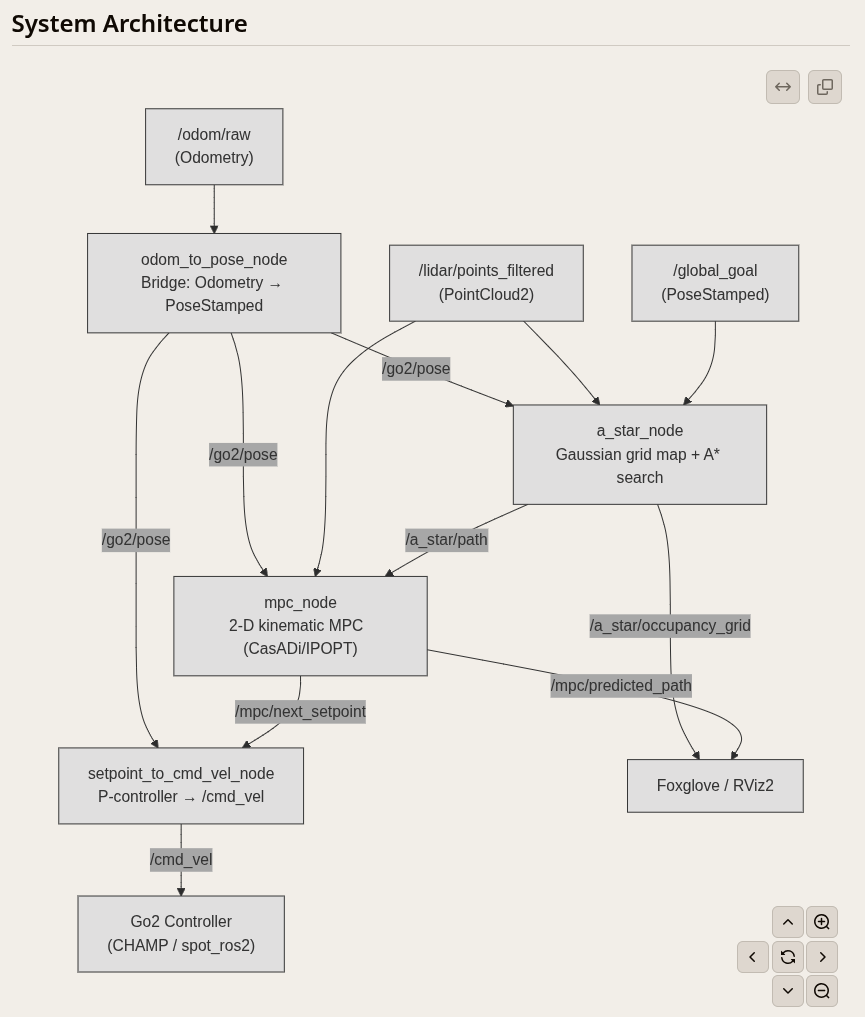
\includegraphics[width=0.86\textwidth]{system_architecture.png}
%   \caption{Architecture of the navigation stack. The two runtime optimization programs analysed in this
%   report are the \astar{} search on the Gaussian occupancy grid and the nonlinear MPC tracker; the Bayesian
%   tuning stage is executed offline and only produces the weight vector $\hat\theta$.}
%   \label{fig:arch}
% \end{figure}

Two design decisions shape everything that follows. First, the locomotion layer is treated as an ideal
velocity-tracking device with a time constant: the report never models legs, contacts or gait, and the robot
is abstracted as a planar holonomic agent, Sections~\ref{sec:platforms} and~\ref{sec:lowlevel} describe
what that layer actually does on each of the two platforms, and why the same abstraction survives the
difference between them. Second, the map is \emph{local and volatile}. The
occupancy grid covers a fixed $10\times10$~m window centred on the robot and is rebuilt from scratch at every
planning cycle, so the planning problem is genuinely map-free, and the geometric reference the MPC tracks is
only valid for one grid width ahead. Section~\ref{sec:localmin} measures what this choice costs, and
Section~\ref{sec:memoryfix} what it takes to repair it.

\subsection{The controlled platforms}
\label{sec:platforms}

The same stack drives two machines whose mechanics could hardly be more different: a Unitree Go2 quadruped
(Fig.~\ref{fig:platforms}\subref{fig:platform-go2}) and a Unitree G1 humanoid
(Fig.~\ref{fig:platforms}\subref{fig:platform-g1}). The Go2 has
twelve actuated joints, three per leg; the G1 has twenty-nine, of which the locomotion layer of
Section~\ref{sec:g1rl} drives fifteen, the twelve leg joints and the three waist joints --- while the arms
are held at a fixed posture. Neither joint set is ever addressed by the controller of this report. Both
platforms are commanded through the same channel, a body-frame twist
$u=(v_x^{\mathrm{cmd}},v_y^{\mathrm{cmd}},\omega^{\mathrm{cmd}})$, and both carry a 3-D LiDAR whose returns
are the only exteroceptive input of the stack. Table~\ref{tab:platforms} collects what distinguishes them
from the controller's point of view; everything else about the two robots is, by construction, invisible to
it.

\begin{figure}[htbp]
  \centering
  \subfloat[Unitree Go2 quadruped\label{fig:platform-go2}]{%
    \begin{minipage}{0.47\textwidth}\centering
      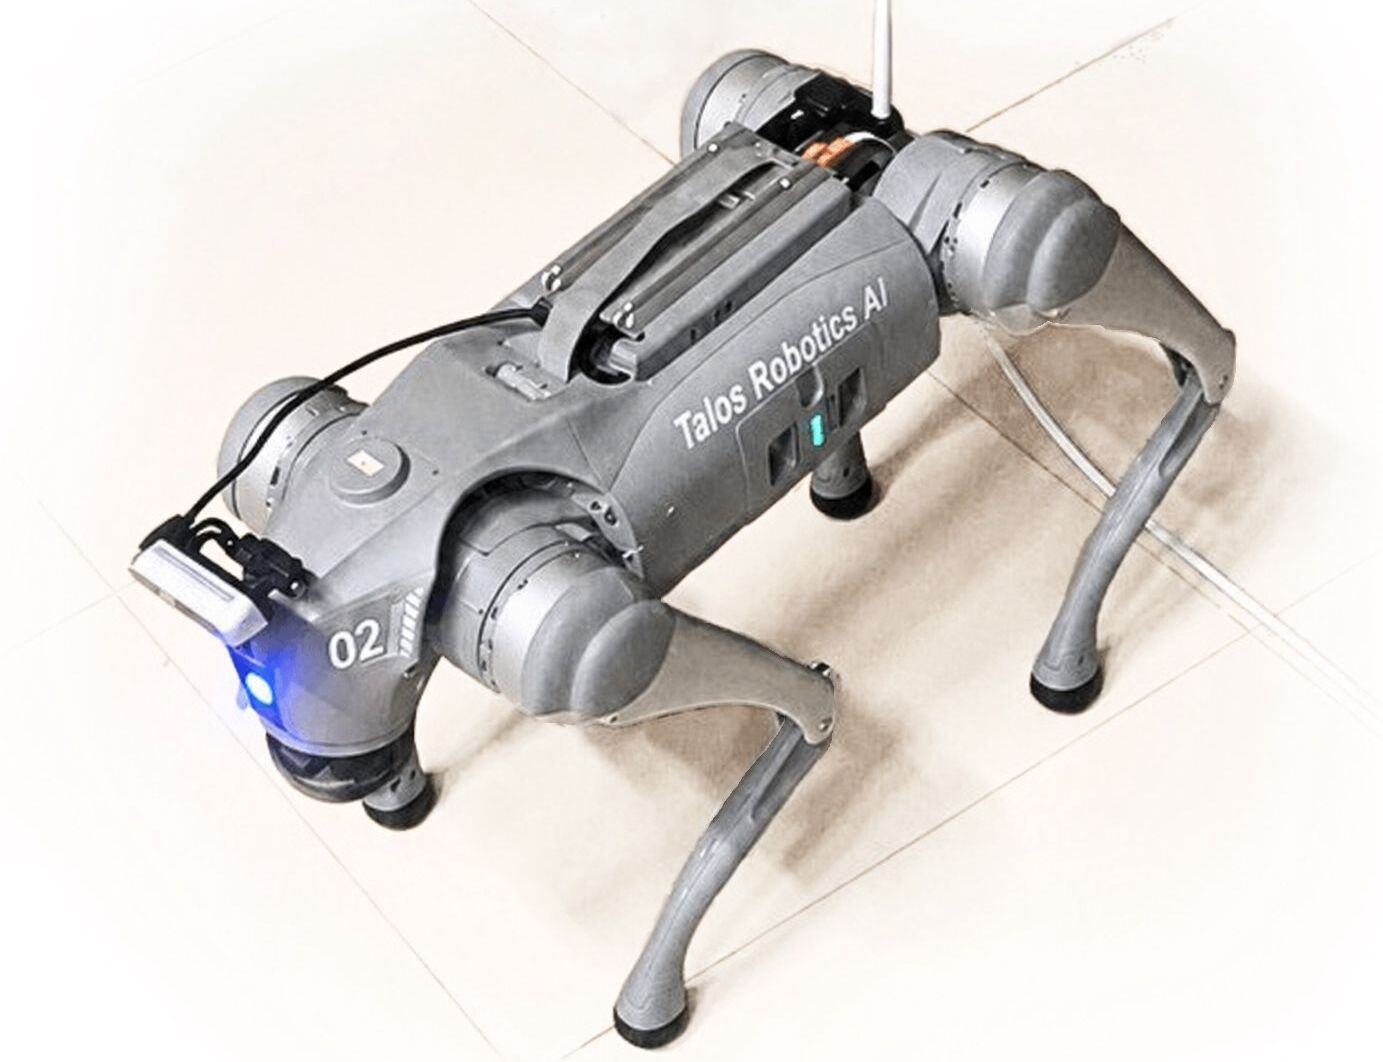
\includegraphics[width=\linewidth]{robot.jpeg}
    \end{minipage}}
  \hfill
  \subfloat[Unitree G1 humanoid\label{fig:platform-g1}]{%
    \begin{minipage}{0.47\textwidth}\centering
      \gonephoto
    \end{minipage}}
  \caption{The two platforms on which the same navigation stack is deployed. (a) The Go2 quadruped, which
  produced all the recorded runs of Section~\ref{sec:hardware}, with its LiDAR mounted on the head. (b) The G1
  humanoid, to which the stack was ported without changing the optimization program: only the constants of the
  actuator-lag model~\eqref{eq:lagcont} and the command mapping of Section~\ref{sec:g1rl} differ.}
  \label{fig:platforms}
\end{figure}

\begin{table}[htbp]
  \centering
  \small
  \caption{The two platforms as the controller sees them. The rows above the rule are properties of the
  machine, those below are properties of the locomotion layer that receives the MPC command; the last row is
  the only one that enters the optimization program, through the prediction model~\eqref{eq:lagcont}. The two
  time constants were identified on the Go2 (Section~\ref{sec:model}) and carried over unchanged to the G1,
  which is the concrete form the ``robot-agnostic'' claim takes.}
  \label{tab:platforms}
  \begin{tabular}{lll}
    \toprule
                                  & Unitree Go2                     & Unitree G1 \\
    \midrule
    Morphology                    & quadruped                       & humanoid \\
    Actuated joints               & $12$ ($3$ per leg)              & $29$ ($15$ driven by the gait policy) \\
    Exteroception                 & Unitree L1 LiDAR                & Livox MID-360 LiDAR \\
    \midrule
    Locomotion layer              & CHAMP gait controller           & AMO reinforcement-learning policy \\
                                  & (vendor sport mode on hardware) & \\
    Layer update rate             & $200$~Hz                        & $50$~Hz \\
    Command interface             & body-frame twist $u$            & body-frame twist $u$, remapped \\
                                  &                                 & (Section~\ref{sec:g1rl}) \\
    Abstraction used by the MPC   & \multicolumn{2}{c}{first-order velocity lag, $\tau_v=0.12$~s, $\tau_w=0.10$~s} \\
    \bottomrule
  \end{tabular}
\end{table}

\subsection{Low-level locomotion layers}
\label{sec:lowlevel}

The controller analysed in this report never commands a joint. Its decision variable is a body-frame twist,
and between that twist and the ground sits a platform-specific layer that turns it into joint commands at
$200$~Hz on the Go2 and $50$~Hz on the G1. Only two properties of that layer reach the optimization problem:
the twist is tracked with a first-order lag rather than instantaneously, and the tracking is fast enough,
relative to the $10$~Hz MPC cycle, for the two layers to be designed separately. This section describes the
two locomotion controllers to the depth needed to justify those two properties and no further. Throughout, $q\in\R^{n_j}$
denotes the vector of joint positions ($n_j=12$ on the Go2, $n_j=29$ on the G1), $\mathcal{T}\in\R^{n_j}$ the
vector of joint torques, and $K_P,K_D\succ0$ the diagonal proportional and derivative gain matrices of the
joint-level loop; the symbol $\tau$ is reserved for the actuator time constants of
Section~\ref{sec:model}.

\subsubsection{Model-based gait generation: CHAMP on the Go2}
\label{sec:champ}

CHAMP \cite{champ} is an open-source implementation of the hierarchical trot controller developed for the MIT
Cheetah \cite{lee2013hierarchical,hyun2014trot}. It is a purely feedforward pipeline: a pattern modulator
imposes the footfall sequence, a trajectory planner turns each leg's phase into a foot position, inverse
kinematics (IK) turns that position into joint angles, and a joint-level impedance loop tracks them.\footnote{On
the physical Go2 the same body-twist interface is served by Unitree's built-in sport-mode controller, which is
closed-source; CHAMP is the locomotion layer of the simulated robot, and the one whose structure can be
stated. The distinction does not reach the MPC: both accept a twist and return trunk motion, and it is only
that input--output behaviour that Section~\ref{sec:model} models.}

\paragraph{Pattern modulation.} Let $t$ denote time. Each leg $i\in\{\mathrm{LF},\mathrm{RF},\mathrm{LH},
\mathrm{RH}\}$ carries a normalised stride clock
\begin{equation}
  \zeta_i(t)=\left(\frac{t}{\Tstr}-\zeta_i^{0}\right)\bmod 1\in[0,1),
  \qquad \Tstr=\Tst+\Tsw ,
  \label{eq:gaitphase}
\end{equation}
where $\Tst$ and $\Tsw$ are the stance and swing durations and $\zeta_i^{0}$ is the phase offset of leg $i$.
Leg $i$ is in stance while $\zeta_i<\beta$ and in swing otherwise, with duty factor $\beta=\Tst/\Tstr$. The
deployed configuration uses $\Tst=\Tsw=0.25$~s, hence $\Tstr=0.5$~s and $\beta=0.5$, and
$\zeta^{0}=(0,\tfrac12,\tfrac12,0)$: the diagonal pairs move together, which is the trot.

\paragraph{Where the command enters.} The commanded twist does not act on the legs directly; it acts on the
\emph{step geometry}, through the Raibert foot-placement heuristic \cite{raibert1986legged}: a foot is placed
half a step ahead of its nominal position, so that sweeping backwards during the stance interval $\Tst$
displaces the trunk by exactly the commanded amount. Let $\bar\pf_i\in\R^3$ be the nominal (zero-command)
position of foot $i$ in the body frame. Translating the nominal stance by the half-step
$\tfrac{1}{2}\Tst\,(v_x^{\mathrm{cmd}},v_y^{\mathrm{cmd}},0)^{\!\top}$ and rotating it about the vertical axis
by the half-stance yaw $\chi_g$ gives the foot displacement
\begin{equation}
  \Delta\pf_i \;=\; R_z(\chi_g)\Big(\bar\pf_i+\tfrac{1}{2}\Tst\,
                  \big(v_x^{\mathrm{cmd}},v_y^{\mathrm{cmd}},0\big)^{\!\top}\Big)-\bar\pf_i ,
  \qquad
  \chi_g = 2\sin\!\Big(\tfrac{1}{4}\Tst\,\omega^{\mathrm{cmd}}\Big)\approx\tfrac{1}{2}\Tst\,\omega^{\mathrm{cmd}} ,
  \label{eq:raibert}
\end{equation}
with $R_z(\cdot)$ the elementary rotation about the vertical axis.\footnote{The implementation obtains
$\chi_g$ from the tangential half-step $\tfrac12\Tst\,\omega^{\mathrm{cmd}}d_c$, with $d_c$ the horizontal
distance from the trunk centre to the nominal foot; $d_c$ cancels, leaving~\eqref{eq:raibert}. The small-angle
form on the right is the yaw swept in half a stance interval, as expected.} The step length and the heading of
the foot trajectory of leg $i$ follow as
\begin{equation}
  L_i = 2\big\|\Delta\pf_i\big\|_2 ,
  \qquad
  \chi_i=\operatorname{atan2}\big(\Delta\pf_{i,y},\,\Delta\pf_{i,x}\big),
  \label{eq:steplen}
\end{equation}
the factor $2$ turning the half-step into the full stride of the foot. Equations~\eqref{eq:raibert} and
\eqref{eq:steplen} are the whole of the command path: the three numbers the MPC publishes are compressed into
one length and one angle per leg, and nothing else of the command reaches the robot.

\paragraph{Foot trajectories and impedance.} With phase and step length fixed, each foot follows a planar
curve in its own trajectory frame, rotated by $\chi_i$ and added to the nominal stance:
$\pf_i=\bar\pf_i+(\,\xi\cos\chi_i,\ \xi\sin\chi_i,\ \eta\,)^{\!\top}$, where $\xi$ and $\eta$ are the
longitudinal and vertical coordinates of the curve. In stance, parametrised by the normalised stance phase
$\zeta_i^{\mathrm{st}}=\zeta_i/\beta\in[0,1)$, the foot sweeps backwards along a shallow arc that presses into
the ground by $h_{\mathrm{st}}$,
\begin{equation}
  \xi=\tfrac{L_i}{2}\left(1-2\zeta_i^{\mathrm{st}}\right),\qquad
  \eta=-h_{\mathrm{st}}\cos\!\left(\frac{\pi\,\xi}{L_i}\right);
  \label{eq:stance}
\end{equation}
in swing, parametrised by $\zeta_i^{\mathrm{sw}}=(\zeta_i-\beta)/(1-\beta)\in[0,1)$, it follows a Bézier curve
of degree $11$ through twelve control points $b_j\in\R^2$,
\begin{equation}
  (\xi,\eta)=\sum_{j=0}^{11}\binom{11}{j}
             \big(\zeta_i^{\mathrm{sw}}\big)^{j}\big(1-\zeta_i^{\mathrm{sw}}\big)^{11-j}\,b_j ,
  \label{eq:swing}
\end{equation}
whose horizontal spread is scaled by $L_i$ and whose vertical spread is scaled by the swing height
$h_{\mathrm{sw}}$. Figure~\ref{fig:gaitparams} collects these quantities on a single leg. The deployed gait uses $h_{\mathrm{sw}}=0.04$~m, $h_{\mathrm{st}}=0.01$~m and a nominal
trunk height $h_0=0.225$~m. A closed-form IK then maps each foot position to the three joint angles of its
leg, $q_i^{\mathrm{ref}}=\mathrm{IK}_i(\pf_i)$, and a proportional--derivative (PD) law closes the loop at the
joints,
\begin{equation}
  \mathcal{T}_i = K_P\big(q_i^{\mathrm{ref}}-q_i\big)+K_D\big(\dot q_i^{\mathrm{ref}}-\dot q_i\big)
  \;=\;\bm{J}_i(q_i)^{\!\top}F_i ,
  \label{eq:impedance}
\end{equation}
where $\bm{J}_i$ is the foot Jacobian of leg $i$, set in bold to distinguish it from the MPC cost $J$ and
from the tuning objective $\mathcal{J}$ of Section~\ref{sec:bo} and $F_i$ the equivalent force at the
foot. Read from right to left, \eqref{eq:impedance} is the point of the architecture: a joint-space PD loop
realises a virtual spring--damper at the foot, of Cartesian stiffness
$\bm{J}_i^{-\top}K_P\bm{J}_i^{-1}$, so the leg absorbs terrain irregularity and impact by
programmable compliance rather than by contact sensing or force control. This is what makes an open-loop gait
generator survive on a real robot.

\begin{figure}[htbp]
  \centering
  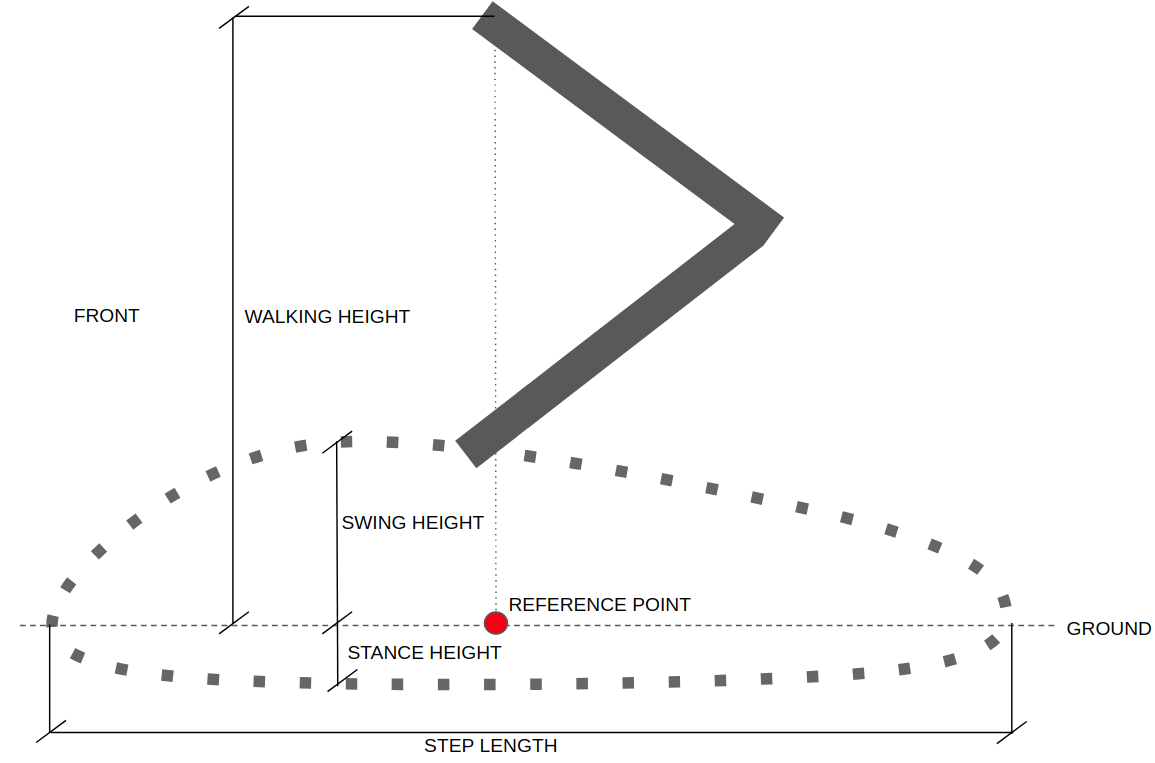
\includegraphics[width=0.72\textwidth]{gait_parameters.png}
  \caption{Geometry of the CHAMP gait on a single leg, seen from the side. The dotted closed curve is the
  cycle described by the foot in its trajectory frame: the upper branch is the swing
  Bézier~\eqref{eq:swing}, which clears the ground by the swing height $h_{\mathrm{sw}}$, and the lower branch
  is the stance arc~\eqref{eq:stance}, which presses into the ground by the stance height $h_{\mathrm{st}}$
  and sweeps backwards to carry the trunk forward. The horizontal extent of the cycle is the step length
  $L_i$ of~\eqref{eq:steplen}, the only channel through which the commanded twist reaches the leg; the
  reference point on the ground line is the nominal stance position $\bar\pf_i$ about which the Raibert
  half-step~\eqref{eq:raibert} displaces the cycle, and the walking height is the nominal trunk height $h_0$.
  Adapted from the CHAMP documentation \cite{champ}.}
  \label{fig:gaitparams}
\end{figure}

\paragraph{Why this layer looks like a lag.} Three consequences propagate upstream, and they are the reason
the model of Section~\ref{sec:model} has the form it has. First, the twist enters only through the step
geometry~\eqref{eq:steplen}: no measured trunk velocity is fed back, so the layer is a feedforward map and the
trunk velocity approaches the commanded one over roughly one stride rather than immediately. Second, that
step geometry is re-evaluated only once per stride, so a command that changes faster than $1/\Tstr=2$~Hz is
averaged, not tracked; a first-order lag with $\tau_v=0.12$~s reaches $98\%$ of its final value in
$4\tau_v\approx\Tstr$, which is why the one-parameter fit of Section~\ref{sec:model} describes the layer as
well as it does. Third, the gait applies its own saturation, $|v_x^{\mathrm{cmd}}|\le0.3$~m/s,
$|v_y^{\mathrm{cmd}}|\le0.25$~m/s and $|\omega^{\mathrm{cmd}}|\le0.5$~rad/s in the deployed configuration.

\subsubsection{Learned whole-body control: the AMO policy on the G1}
\label{sec:g1rl}

On the humanoid the same interface is produced by a neural network instead of a gait generator. The deployed
controller is AMO (Adaptive Motion Optimization) \cite{li2025amo}, a reinforcement-learning (RL) policy
trained in simulation for the G1 and its twenty-nine degrees of freedom (DoF). AMO is deliberately \emph{not} a walking controller: it is a
loco-manipulation policy, trained to track torso height, torso orientation and upper-body targets while
walking, on a hybrid dataset in which an offline trajectory-optimization module supplies whole-body
references that are kinematically consistent with the commanded end-effector motion. The navigation stack
exercises only its locomotion subset, the arms are held at the default posture and only the base command
is driven, but the policy is the one trained for the larger task, which is what makes the same platform
usable for manipulation later without changing the layer the MPC talks to.

\paragraph{Structure.} At each tick $k$ of the $50$~Hz policy loop, the network maps an observation to an
action,
\begin{equation}
  a_k=\pi(o_k)\in\R^{15},
  \qquad
  o_k=\big(\,\omega^{\mathrm{b}}_k,\ \hat g_k,\ \tilde u_k,\ q_k-\qdef,\ \dot q_k,\ a_{k-1}\,\big),
  \label{eq:rlpolicy}
\end{equation}
where $\omega^{\mathrm{b}}_k\in\R^3$ is the body angular velocity, $\hat g_k\in\R^3$ the gravity direction
expressed in the body frame (the tilt an inertial measurement unit (IMU) provides without a global heading), $q_k,\dot q_k$ the
measured joint positions and velocities of the $23$ observed joints, $\qdef$ the default posture,
$a_{k-1}$ the previous action, and $\tilde u_k$ the command. The action is not a torque: it is an offset on
the default posture, which the same joint-level PD law as~\eqref{eq:impedance} converts into torque,
\begin{equation}
  q_k^{\mathrm{ref}}=\qdef+s_a\,a_k,
  \qquad
  \mathcal{T}_k=K_P\big(q_k^{\mathrm{ref}}-q_k\big)+K_D\big(0-\dot q_k\big),
  \label{eq:rlpd}
\end{equation}
with $s_a$ a fixed action scale and a zero reference joint velocity. The learned part of the controller is
therefore exactly the map from observation to PD setpoint; the stabilising loop underneath it is the same
fixed impedance as on the quadruped. The policy $\pi$ is obtained by proximal policy optimization (PPO)
\cite{schulman2017ppo}, maximising the expected discounted return
$\mathbb{E}\big[\sum_k\gamma^k\mathcal{R}_k\big]$ with $\gamma\in(0,1)$ and a stage reward $\mathcal{R}_k$
that pays for tracking the commanded twist and penalises posture deviation, joint effort and action rate;
masses, friction, gains and latencies are randomised during training so that the fixed policy transfers to
hardware \cite{rudin2022walk}.

% \paragraph{The command mapping.} The command handed to the network is not the MPC twist but its image under a
% calibrated map, $\tilde u_k=\mathcal{M}(u_k)$, and that map is not a change of units. The policy's yaw channel
% is a heading \emph{offset} saturating at $\pm0.2$~rad rather than a yaw rate, its lateral channel uses the
% opposite sign convention, and the policy plants its feet whenever all three channels fall below a stand gate
% of about $0.1$ of full scale. The constants of $\mathcal{M}$ were identified so that the achieved twist
% matches the commanded one to within $10\%$ over the operating range. The stand gate is the one visible
% unmodelled nonlinearity of the cascade: a near-pure rotation in place, which the MPC produces when the
% reference turns sharply at low speed, falls below it and returns no motion at all.

\subsubsection{The cascade and its abstraction seam}
\label{sec:cascade}

Fig.~\ref{fig:cascade} places the two locomotion layers in the control structure they belong to. The stack is
a cascade of four loops whose rates are separated by roughly a decade each: the \astar{} reference is
recomputed at $1$~Hz, the MPC at $10$~Hz, the locomotion layer at $50$--$200$~Hz, and the joint PD loop at the
motor-driver rate. That separation is the standard justification for designing each layer against a static
abstraction of the one below it, and the abstraction used here is deliberately minimal: three decoupled
first-order lags, Eq.~\eqref{eq:lagcont}, whose time constants are identified in Section~\ref{sec:model}. Both
locomotion layers, the hand-designed one and the learned one, are approximated by the same two numbers.

% This is the entire content of the ``robot-agnostic'' claim, and it is worth stating what it costs. The
% abstraction discards leg dynamics, contact, footstep timing and the two nonlinearities named above --- the
% gait saturation of Section~\ref{sec:champ} and the stand gate of Section~\ref{sec:g1rl}. What survives is a
% question of degree rather than of principle, and Section~\ref{sec:mismatch} answers it quantitatively by
% inflating the plant lags by $60$--$67\%$ against the model and measuring what the closed loop loses.

\begin{figure}[htbp]
  \centering
  \begin{tikzpicture}[
    font=\footnotesize,
    >={Latex[length=1.8mm]},
    blk/.style={draw, rounded corners=3pt, align=center, inner sep=5pt, minimum height=8mm,
                fill=black!3},
    hlblk/.style={draw=bluePoli, line width=0.9pt, rounded corners=3pt, align=center, inner sep=5pt,
                  minimum height=8mm, fill=bluePoli!10},
    sig/.style={->, semithick},
    sl/.style={font=\scriptsize, inner sep=2.2pt},
  ]
    % ------------------------------------------------------------------ planning
    \node[blk,  text width=46mm] (astar) at (0,6.1) {\astar{} search on the occupancy grid\\$1$~Hz};
    \node[hlblk,text width=46mm] (mpc)   at (0,4.1) {nonlinear MPC tracker\\$10$~Hz};

    \draw[sig] (0,7.15) -- node[sl,right] {goal $x_g$} (astar.north);
    \draw[sig] (astar) -- node[sl,right] {$x^{\mathrm{ref}}$} (mpc);

    % --------------------------------------------------------- locomotion layer
    \coordinate (split) at (0,2.3);
    \node[blk, text width=52mm] (champ) at (-3.8,0.75)
      {\textbf{Go2}: CHAMP gait generator\\
       phase~\eqref{eq:gaitphase} $\to$ step~\eqref{eq:steplen} $\to$ foot~\eqref{eq:swing}\\
       $\to$ IK $\to$ joint PD, $200$~Hz};
    \node[blk, text width=52mm] (rl) at (3.8,0.75)
      {\textbf{G1}: AMO reinforcement-learning policy\\
       $\mathcal{M}\to\pi$~\eqref{eq:rlpolicy} $\to$ PD setpoint~\eqref{eq:rlpd}\\
       $\to$ joint PD, $50$~Hz};
    \node[draw, dashed, rounded corners=4pt, fit=(champ)(rl), inner sep=7pt] (llbox) {};
    \node[sl, anchor=south west] at ([xshift=2pt,yshift=1.5pt]llbox.north west)
      {low-level locomotion layer};

    \draw[sig] (mpc.south) -- node[sl, right, align=left, xshift=1pt]
      {$u=(v_x,v_y,\omega)^{\mathrm{cmd}}$\\ first-order lag~\eqref{eq:lagcont}} (split);
    \draw[sig] (split) -| ([xshift=12mm]champ.north);
    \draw[sig] (split) -| ([xshift=-12mm]rl.north);

    % ------------------------------------------------------------------- plant
    \node[blk, text width=28mm] (robot) at (0,-2.3) {robot $+$ ground};
    \draw[sig] ([xshift=12mm]champ.south) -- (robot.north west);
    \draw[sig] ([xshift=-12mm]rl.south)   -- (robot.north east);
    \node[sl] at (0,-1.35) {$\mathcal{T}$: joint torques};

    % ---------------------------------------------------------------- feedback
    \node[blk, text width=38mm] (est)  at (6.2,4.1) {state estimation (EKF)\\$\hat x$: pose $+$ body twist};
    \node[blk, text width=38mm] (grid) at (6.2,6.1) {Gaussian occupancy grid\\$\mathcal{P}_k$, rebuilt at $1$~Hz};

    \draw[semithick] (robot.east) -- node[sl, above] {LiDAR, IMU, encoders} (9.2,-2.3) -- (9.2,6.1);
    \draw[sig] (9.2,4.1) -- (est.east);
    \draw[sig] (9.2,6.1) -- (grid.east);
    \draw[sig] (est.west)  -- (mpc.east);
    \draw[sig] (grid.west) -- (astar.east);
  \end{tikzpicture}
  \caption{Cascaded structure of the controller, from the goal down to joint torques. The
  rates fall by roughly a decade at every seam ($1$~Hz, $10$~Hz, $50$--$200$~Hz, motor-driver rate), which is
  what allows the layers to be designed separately, and the two branches inside the dashed box, a
  hand-designed gait generator and a learned policy, are interchangeable precisely because they present the
  same twist interface $u$.}
  \label{fig:cascade}
\end{figure}

\subsection{Environment representation}
\label{sec:grid}

Let $\mathcal{P}_k=\{p_i\in\R^3\}_{i=1}^{N_k}$ be the LiDAR point cloud available at cycle $k$, projected on
the plane. The grid is a square of side $2h_w$ ($h_w=5$~m) centred on the robot position, discretised with
resolution $\Delta=0.25$~m into $n_c=2h_w/\Delta=40$ cells per axis. The occupancy probability of cell $c$ is
a Gaussian tail of the distance to the nearest return,
\begin{equation}
  P(c) \;=\; 1-\Phi\!\left(\frac{d_{\min}(c,\mathcal{P}_k)}{\sigma}\right),
  \qquad d_{\min}(c,\mathcal{P}_k)=\min_{p\in\mathcal{P}_k}\|c-p\|_2 ,
  \label{eq:grid}
\end{equation}
with $\Phi$ the standard normal cumulative distribution function,
\begin{equation}
  \Phi(x) \;=\; \frac{1}{\sqrt{2\pi}}\int_{-\infty}^{x}e^{-t^2/2}\,\mathrm{d}t
  \;=\; \frac{1}{2}\left(1+\operatorname{erf}\!\left(\frac{x}{\sqrt{2}}\right)\right)\in(0,1),
  \label{eq:phi}
\end{equation}
and $\sigma=0.15$~m. Equation~\eqref{eq:grid} is an \emph{inflation}
model: it is not a Bayesian occupancy update (there is no recursive filtering, no ray casting and no free-space
carving), but a smooth, monotone map from clearance to cost, whose one parameter $\sigma$ sets the width of
the obstacle halo. Cells with $P(c)\ge P_{\mathrm{thr}}=0.4$ are hard obstacles. The left panel of
Fig.~\ref{fig:occprofile} shows the trade-off governed by $\sigma$: a small $\sigma$ leaves doorways open but
hugs walls, a large one closes gaps the robot could physically cross.

Because the grid is rebuilt from scratch, its construction cost is the dominant cost of the planning layer,
$O(n_c^2\,|\mathcal{P}_k|)$; vectorised over $40\times40$ cells and ${\sim}180$ returns it measures
$4$--$5$~ms on average together with the \astar{} search (Section~\ref{sec:setup}), which at the $1$~Hz
replanning rate is negligible against the $10$~Hz MPC.

\begin{figure}[htbp]
  \centering
  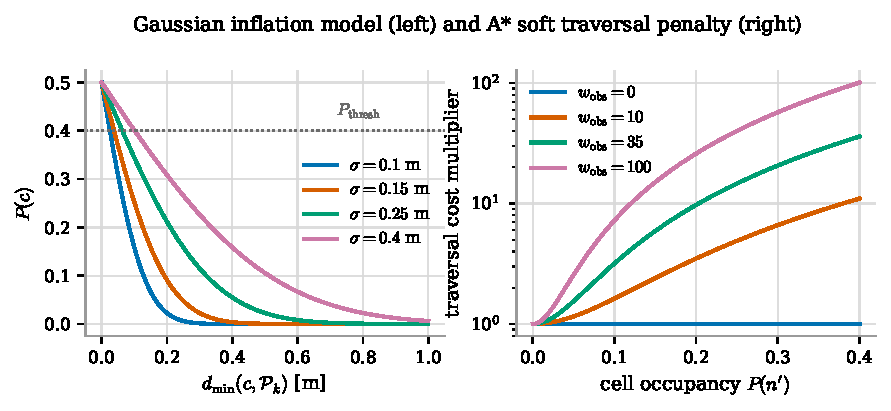
\includegraphics[width=0.92\textwidth]{fig_occupancy_profile.pdf}
  \caption{Left: the Gaussian inflation model~\eqref{eq:grid} for four values of $\sigma$, with the hard
  threshold $P_{\mathrm{thr}}=0.4$. Right: the soft traversal-cost multiplier
  $1+w_{\mathrm{obs}}(P/P_{\mathrm{thr}})^2$ of the \astar{} edge cost~\eqref{eq:astarcost}, which is what
  actually keeps the path away from walls; the deployed value is $w_{\mathrm{obs}}=35$.}
  \label{fig:occprofile}
\end{figure}

\subsection{Plant model and state-space formulation}
\label{sec:model}

The MPC model must predict where the robot will be, not where it was told to go. Commanding a legged platform
a body-frame velocity does not produce that velocity instantaneously: the locomotion controller responds with
a measured time constant of $\tau\approx0.10$--$0.15$~s, which over a $5$~s horizon accumulates into a
prediction error of several tens of centimetres if neglected. The model therefore augments the usual planar
kinematic state with the three velocity states, giving
\begin{equation}
  x \;=\; \begin{bmatrix} p_x & p_y & \psi & v_x & v_y & \omega\end{bmatrix}^{\!\top}\in\R^{6},
  \qquad
  u \;=\; \begin{bmatrix} v_x^{\mathrm{cmd}} & v_y^{\mathrm{cmd}} & \omega^{\mathrm{cmd}}\end{bmatrix}^{\!\top}\in\R^{3},
  \label{eq:state}
\end{equation}
where $(p_x,p_y)$ and $\psi$ are the world-frame pose and $(v_x,v_y,\omega)$ the body-frame twist actually
realised by the platform. In continuous time the actuator behaves as three decoupled first-order lags driven
by the commands,
\begin{equation}
  \dot v_x = \frac{u_1-v_x}{\tau_v},\qquad
  \dot v_y = \frac{u_2-v_y}{\tau_w},\qquad
  \dot \omega = \frac{u_3-\omega}{\tau_w},
  \label{eq:lagcont}
\end{equation}
while the pose obeys the holonomic body-to-world rotation
\begin{equation}
  \dot p_x = v_x\cos\psi - v_y\sin\psi,\qquad
  \dot p_y = v_x\sin\psi + v_y\cos\psi,\qquad
  \dot\psi = \omega .
  \label{eq:kincont}
\end{equation}
The identified constants are $\tau_v=0.12$~s and $\tau_w=0.10$~s.
% \footnote{In the deployed code the lateral
% velocity $v_y$ is propagated with $\tau_w$ rather than $\tau_v$, i.e.\ lateral motion is assumed to respond as
% fast as yaw. The two constants differ by $20$~ms, well inside the identification uncertainty, so the
% substitution is numerically immaterial; it is reported here because the analysis reproduces the deployed
% formulation exactly rather than an idealisation of it.}

Model~\eqref{eq:lagcont}--\eqref{eq:kincont} is holonomic: unlike a differential-drive vehicle, the platform
can command a lateral velocity, so no nonholonomic constraint appears and the input set is a box. This is what
makes the resulting NLP comparatively benign, the nonlinearity is confined to the rotation
$R(\psi)$ and to the obstacle distances.

Fig.~\ref{fig:lag} quantifies why the lag states are worth their computational cost. The left panel compares
the true velocity response with the instantaneous model $v\equiv u$ for a step command; the right panel
integrates the resulting velocity discrepancy over one $5$~s horizon and reports the peak position error as a
function of $\tau_v$.
% At the identified $\tau_v=0.12$~s the instantaneous model mispredicts the horizon
% end-point by ${\sim}7$~cm, which is of the same order as the tracking accuracy the controller is asked to
% deliver.

\begin{figure}[htbp]
  \centering
  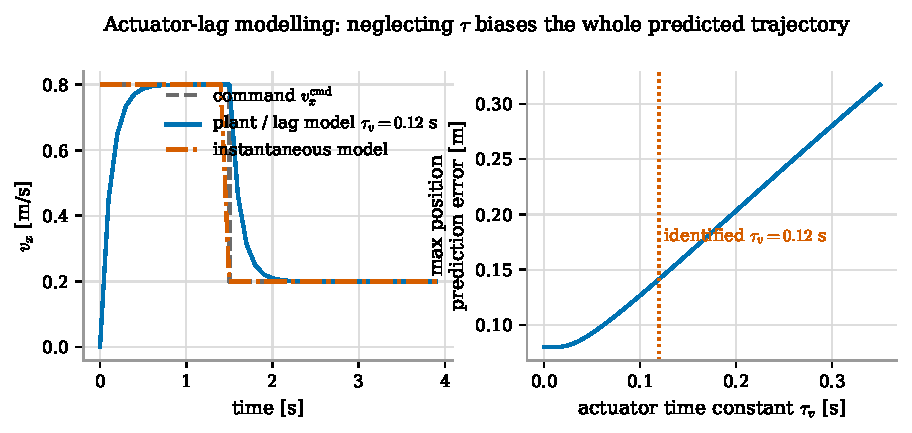
\includegraphics[width=0.92\textwidth]{fig_lag_model.pdf}
  \caption{Actuator-lag modelling. Left: response of the first-order-lag model~\eqref{eq:lagcont} against the
  instantaneous model $v\equiv u$ for a step in commanded forward velocity. Right: maximum position
  prediction error accumulated over one $5$~s horizon by neglecting the lag, as a function of $\tau_v$.}
  \label{fig:lag}
\end{figure}

\subsection{Navigation problem statement}
\label{sec:statement}

Let $x_g\in\R^2$ be the goal. The navigation task is the receding-horizon optimal control problem
\begin{subequations}
\label{eq:ocp}
\begin{align}
  \min_{u_0,\dots,u_{N-1}}\;\; & J\!\left(x_{0:N},u_{0:N-1},\mathcal{P}_k,\theta\right) \label{eq:ocp-cost}\\
  \text{s.t.}\quad & x_{t+1}=f(x_t,u_t), && t=0,\dots,N-1, \label{eq:ocp-dyn}\\
                   & x_0 = \hat x(t_k), \label{eq:ocp-init}\\
                   & u_t\in\mathcal{U}, && t=0,\dots,N-1, \label{eq:ocp-input}\\
                   & d\!\left(x_t,\mathcal{P}_k\right)\ge r_{\min}, && t=0,\dots,N, \label{eq:ocp-obs}
\end{align}
\end{subequations}
solved at every sampling instant $t_k$, of which only $u_0$ is applied. Three features of~\eqref{eq:ocp}
determine the whole design:

\begin{itemize}
  \item \textbf{The goal is not reachable within the horizon.} With $N\Delta t=5$~s and a cruise speed of
        $0.5$~m/s the horizon spans $2.5$~m, while the goal may be tens of metres away and outside the
        sensed region altogether. The cost~\eqref{eq:ocp-cost} therefore cannot be a distance to $x_g$; it
        must be a distance to a \emph{reference trajectory} produced by a separate, cheaper program that
        looks further ahead. That program is the \astar{} search of Section~\ref{sec:astar}.
  \item \textbf{The obstacle set is a point cloud, not a polytope.} Constraint~\eqref{eq:ocp-obs} is
        non-convex, and its description changes at every cycle. It is relaxed into a smooth penalty
        (Section~\ref{sec:barrier}), which keeps the NLP smooth and always feasible at the price of losing
        the hard safety guarantee.
  \item \textbf{The cost is parametrised by $\theta$.} The eleven weights in $\theta$ are not physical
        quantities; they are design variables of a second-level optimization problem
        (Section~\ref{sec:bo}).
\end{itemize}

%=============================================================================
\section{Formulation of the optimization program}
\label{sec:formulation}

\subsection{Reference generation: \astar{} as a discrete program}
\label{sec:astar}

At every planning tick the geometric reference is the solution of a shortest-path problem on the
$8$-connected grid of Section~\ref{sec:grid}. Cells with $P\ge P_{\mathrm{thr}}$ are removed from the graph;
the remaining edges carry the cost
\begin{equation}
  g(n\rightarrow n') \;=\; c_{\mathrm{move}}\cdot\Delta\cdot
  \left[1+w_{\mathrm{obs}}\left(\frac{P(n')}{P_{\mathrm{thr}}}\right)^{\!2}\right],
  \qquad c_{\mathrm{move}}\in\{1,\sqrt2\},
  \label{eq:astarcost}
\end{equation}
with $w_{\mathrm{obs}}=35$. The normalised quadratic in~\eqref{eq:astarcost} is the mechanism that produces
medial-axis-like paths: a cell just below the hard threshold costs $36\times$ an open cell, so the search
prefers the middle of a corridor over the short path that grazes a wall, yet a doorway is never closed
outright. The heuristic
\begin{equation}
  h(n) \;=\; \Delta\sqrt{(i_x-g_x)^2+(i_y-g_y)^2}
  \label{eq:astarh}
\end{equation}
is admissible because the bracket in~\eqref{eq:astarcost} is bounded below by $1$, so no edge can ever be
cheaper than its Euclidean length; the search is therefore an exact \astar{} and returns a cost-optimal path
on the current grid. Diagonal expansions are additionally rejected when either of the two orthogonal
neighbours is blocked, which prevents the path from squeezing through a gap of zero width that the physical
body cannot cross.

\paragraph{Rolling horizon.} Because the grid is local, the \astar{} target is
\begin{equation}
  x_{\mathrm{local}} \;=\;
  \begin{cases}
    \mathrm{cell}(x_g), & x_g\in\mathrm{grid},\\[2pt]
    \mathrm{ray}(x_0\!\rightarrow\! x_g)\cap\partial\,\mathrm{grid}, & \text{otherwise},
  \end{cases}
  \label{eq:localgoal}
\end{equation}
i.e.\ when the goal is out of the window the planner aims at the boundary cell along the ray to the goal,
advancing one grid width at a time. If the selected cell is occupied, a breadth-first search returns the
nearest free cell, so \astar{} always receives a valid target. The resulting grid path is resampled at
$\Delta s=0.15$~m and smoothed with a $7$-tap moving average (endpoints preserved) to remove the
grid-induced zig-zag before it is handed to the MPC.

Equation~\eqref{eq:localgoal} is a greedy, purely reactive rule, and it is the single most consequential
approximation in the stack: the ray to the goal carries no information about the free-space topology, so a
wall that separates the robot from the goal is re-discovered at every cycle and never remembered.
Section~\ref{sec:localmin} shows the resulting livelock in a two-room world, and
Section~\ref{sec:memoryfix} repairs it by replacing the ray with the shortest path on the \emph{remembered}
map --- of which~\eqref{eq:localgoal} is exactly the empty-memory special case.

\begin{figure}[htbp]
  \centering
  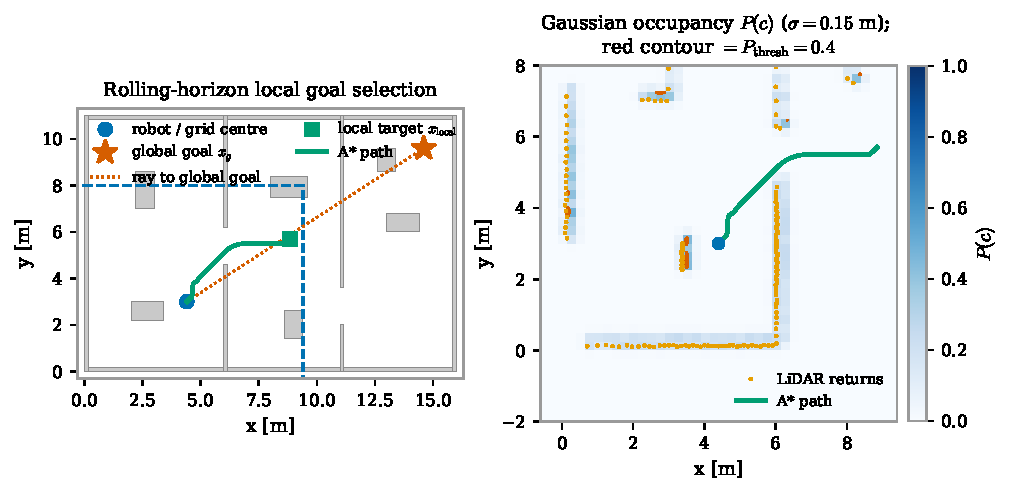
\includegraphics[width=\textwidth]{fig_grid_astar.pdf}
  \caption{Left: rolling-horizon target selection~\eqref{eq:localgoal} --- the dashed square is the
  $10\times10$~m local grid, the dotted line the ray to the global goal, the square marker the local target
  where that ray meets the grid boundary, and the solid line the \astar{} solution. Right: the Gaussian
  occupancy field~\eqref{eq:grid} built from the current returns, with the $P=0.4$ hard-obstacle contour.}
  \label{fig:gridastar}
\end{figure}

\subsection{Model discretization}
\label{sec:discretization}

With sampling time $\Delta t$, the lag subsystem~\eqref{eq:lagcont} is linear and time-invariant, so it is
discretised \emph{exactly} under a zero-order-hold input. Defining
\begin{equation}
  \lambda_v = 1-e^{-\Delta t/\tau_v},\qquad \lambda_w = 1-e^{-\Delta t/\tau_w},
  \label{eq:lags}
\end{equation}
the velocity update is the exact solution of~\eqref{eq:lagcont} over one step,
\begin{equation}
  v_{x,k+1}=(1-\lambda_v)v_{x,k}+\lambda_v u_{1,k},\qquad
  v_{y,k+1}=(1-\lambda_w)v_{y,k}+\lambda_w u_{2,k},\qquad
  \omega_{k+1}=(1-\lambda_w)\omega_{k}+\lambda_w u_{3,k}.
  \label{eq:veldisc}
\end{equation}
The pose is then integrated with one forward-Euler step, but evaluated on the \emph{post-lag} velocity:
\begin{equation}
  \begin{aligned}
    p_{x,k+1} &= p_{x,k} + \left(v_{x,k+1}\cos\psi_k - v_{y,k+1}\sin\psi_k\right)\Delta t,\\
    p_{y,k+1} &= p_{y,k} + \left(v_{x,k+1}\sin\psi_k + v_{y,k+1}\cos\psi_k\right)\Delta t,\\
    \psi_{k+1} &= \psi_k + \omega_{k+1}\Delta t .
  \end{aligned}
  \label{eq:posedisc}
\end{equation}
Using $v_{k+1}$ instead of $v_k$ in~\eqref{eq:posedisc} is a semi-implicit (symplectic-Euler) choice: it costs
nothing, removes the one-step delay that explicit Euler would introduce between a command and the predicted
displacement, and makes the discrete model reproduce the measured step response of the platform. Equations
\eqref{eq:veldisc}--\eqref{eq:posedisc} define the map $x_{k+1}=f(x_k,u_k)$ used in~\eqref{eq:ocp-dyn}. Only
$\cos\psi_k$, $\sin\psi_k$ and the obstacle distances are nonlinear; $f$ is $C^\infty$ and its Jacobian is
sparse and analytically available through CasADi's algorithmic differentiation.

\subsection{The nonlinear MPC program}
\label{sec:nlp}

\subsubsection{Decision variables and cost}
\label{sec:cost}

The NLP is written in the \emph{simultaneous} (direct multiple-shooting with a full state parametrisation)
form: both the state and the input sequences are decision variables and the dynamics enter as equality
constraints,
\begin{equation}
  z \;=\; \big(X,U\big),\qquad X=[x_0,\dots,x_N]\in\R^{6\times(N+1)},\quad U=[u_0,\dots,u_{N-1}]\in\R^{3\times N}.
\end{equation}
This is the standard choice for interior-point solvers: it keeps the Jacobian sparse and banded, whereas a
condensed single-shooting formulation would produce a small but dense problem with a much worse conditioned
Hessian over a $50$-step horizon.

With $e_k=x_k-x_{\mathrm{ref},k}$ the cost is
\begin{equation}
  J(z;\theta) \;=\;
  \underbrace{\sum_{k=0}^{N-1}\Big[e_k^{\!\top} Q\, e_k
  \;+\; u_k^{\!\top} R\, u_k
  \;+\; \Rjerk\|u_k-u_{k-1}\|_2^2
  \;+\; \Jobs(x_k)\Big]}_{\text{stage cost}}
  \;+\;\underbrace{e_N^{\!\top} Q_T\, e_N + \Jobs(x_N)}_{\text{terminal cost}},
  \label{eq:cost}
\end{equation}
with
\begin{equation}
  Q=\mathrm{diag}(Q_x,\,Q_y,\,Q_\psi,\,0,\,0,\,0),\qquad
  Q_T=\rho\,Q,\qquad
  R=\mathrm{diag}(R_{v_x},R_{v_y},R_\omega).
  \label{eq:weights}
\end{equation}
Three properties of~\eqref{eq:cost}--\eqref{eq:weights} deserve comment.

\emph{The stage weight is only semi-definite.} No velocity state is penalised: $Q$ has rank $3$ out of $6$.
The velocities are shaped indirectly, through the lag dynamics and through the input penalty $R$. This keeps
the reference generator simple --- an \astar{} path carries no velocity information --- but it removes any
direct damping of the velocity states from the cost, and it is the reason why the Riccati comparison of
Section~\ref{sec:terminal} requires a regularisation.

\emph{The rate penalty couples consecutive inputs.} The term $\Rjerk\|u_k-u_{k-1}\|^2$ (with $u_{-1}$ the
previously applied command) is the discrete analogue of an input-rate penalty. It is the only term that
introduces off-diagonal blocks between adjacent input stages in the Hessian, and its purpose is physical: a
legged platform tracks a smooth velocity profile far better than a chattering one.

\emph{The terminal cost is a scaled copy of the stage cost.} $Q_T=\rho Q$ with $\rho=Q_{\mathrm{terminal}}$ is
a heuristic, not a Lyapunov function: it is neither the solution of a Riccati equation nor an exact
cost-to-go, and it acts only on the three position/heading components. Section~\ref{sec:terminal} quantifies
the gap.

\subsubsection{Obstacle avoidance as a smooth barrier}
\label{sec:barrier}

The hard clearance constraint~\eqref{eq:ocp-obs} is replaced by a penalty evaluated on the $M$ nearest LiDAR
returns $\{p_j\}_{j=1}^{M}$ inside a search radius of $3$~m:
\begin{equation}
  \Jobs(x_k) \;=\; \Wobs\sum_{j=1}^{M}
  \left[\underbrace{\tfrac12\Big(1-\tanh\big(\tfrac{\aobs}{2}(d_{k,j}-\robs)\big)\Big)}_{\text{soft sigmoid zone}}
  \;+\;\underbrace{2\max\!\big(0,\;\robs-d_{k,j}\big)^2}_{\text{quadratic penetration penalty}}\right],
  \label{eq:barrier}
\end{equation}
\begin{equation}
  d_{k,j}=\sqrt{(p_{x,k}-p_{j,x})^2+(p_{y,k}-p_{j,y})^2+\varepsilon},\qquad \varepsilon=10^{-6}.
  \label{eq:dist}
\end{equation}
The additive constant $\varepsilon$ makes~\eqref{eq:dist} differentiable at zero distance, where the Euclidean
norm is not. The logistic term is written with $\tanh$ rather than as $1/(1+e^{\aobs(d-\robs)})$ because the
two are algebraically identical while the former does not overflow for large arguments.

The hybrid structure of~\eqref{eq:barrier} is deliberate and is best read from Fig.~\ref{fig:barriershape}.
The sigmoid saturates at $\Wobs$ as $d\to0$: on its own it is a \emph{bounded} penalty, so a sufficiently
strong tracking term can always buy its way through an obstacle, and --- worse for the solver --- its gradient
vanishes both far away and deep inside the obstacle, leaving a stationary point precisely where the robot must
be pushed out. The quadratic term $2\max(0,\robs-d)^2$ repairs both defects inside the safety radius: it is
unbounded and its gradient grows linearly with penetration. The price is visible in the third panel: the
curvature of~\eqref{eq:barrier} scales as $\aobs^2\Wobs$, so a steep, heavy barrier injects large, rapidly
varying eigenvalues into the Hessian exactly in the region where the solution lives. This is the conditioning
trade-off measured in Section~\ref{sec:barriersweep}.

\begin{figure}[htbp]
  \centering
  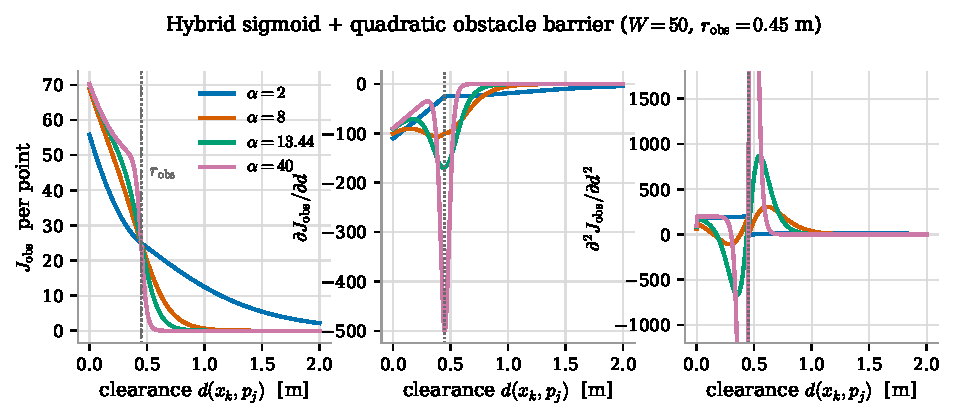
\includegraphics[width=\textwidth]{fig_barrier_shape.pdf}
  \caption{The hybrid barrier~\eqref{eq:barrier} for four steepness values ($\Wobs=50$, $\robs=0.45$~m):
  value (left), gradient (centre) and curvature (right) versus clearance. The sigmoid alone saturates and
  loses its gradient inside the obstacle; the quadratic term restores an unbounded, linearly growing
  restoring force for $d<\robs$. The curvature grows as $\aobs^2$, which is what degrades the conditioning of
  the NLP.}
  \label{fig:barriershape}
\end{figure}

Relaxing a hard constraint into a penalty is a modelling choice with three consequences worth stating
explicitly. \emph{(i)} The NLP is always feasible --- there is no state constraint that can render the
problem infeasible when the robot is already too close to an obstacle, which for a real-time loop with no
fallback trajectory is a significant robustness advantage. \emph{(ii)} Safety is no longer guaranteed:
\eqref{eq:barrier} is not an exact penalty, so a finite $\Wobs$ admits a finite violation. A control-barrier
formulation \cite{ames2019cbf} would recover the guarantee at the price of feasibility and of a much harder
NLP. \emph{(iii)} The barrier is evaluated only at the $N+1$ discrete nodes, so nothing forbids the continuous
inter-sample trajectory from clipping a thin obstacle --- a further reason to keep $\Delta t$ small
(Section~\ref{sec:dtsweep}).

\paragraph{Sentinel padding.} $M=12$ is fixed. When fewer than $M$ returns lie inside the search radius, the
missing rows of the obstacle parameter are filled with a sentinel at $10^3$~m, whose barrier contribution is
numerically zero. This apparently cosmetic detail is what allows the NLP to be built \emph{once}: the number
of terms in~\eqref{eq:barrier}, and therefore the sparsity pattern of the Jacobian and Hessian, never changes
between cycles, so the symbolic factorisation and the warm start remain valid regardless of how cluttered the
scene is.

\subsubsection{Constraints}
\label{sec:constraints}

The program carries only equality constraints and input bounds:
\begin{subequations}
\label{eq:cons}
\begin{align}
  & x_{k+1}-f(x_k,u_k)=0, && k=0,\dots,N-1, \label{eq:cons-dyn}\\
  & x_0-\hat x=0, \label{eq:cons-init}\\
  & 0\;\le\;u_{1,k}\;\le\;v_{x,\max}, && k=0,\dots,N-1, \label{eq:cons-vx}\\
  & |u_{2,k}|\le v_{y,\max},\qquad |u_{3,k}|\le\omega_{\max}, && k=0,\dots,N-1, \label{eq:cons-vyw}
\end{align}
\end{subequations}
with $v_{x,\max}=1.0$~m/s, $v_{y,\max}=0.5$~m/s and $\omega_{\max}=1.5$~rad/s. Three remarks:

\begin{itemize}
  \item \textbf{No state constraints.} Neither the obstacle clearance nor the velocity states are
        constrained; the former is penalised, the latter are bounded implicitly because
        \eqref{eq:veldisc} is a convex combination of a bounded command and the previous velocity, so
        $|v_{x,k}|\le v_{x,\max}$ for all $k$ whenever $|v_{x,0}|\le v_{x,\max}$. The feasible set of the NLP
        is therefore a box intersected with an affine-in-$X$ manifold, and a feasible point is always
        trivially available (integrate any admissible input sequence).
  \item \textbf{Forward velocity is non-negative.} Constraint~\eqref{eq:cons-vx} forbids reversing. This is a
        deployment decision --- the LiDAR field of view and the gait controller both favour forward motion ---
        but it removes the manoeuvre that would resolve a dead end, and it therefore contributes to the
        livelock of Section~\ref{sec:localmin}.
  \item \textbf{Bounds are parameters, not constants.} $v_{x,\max}$, $v_{y,\max}$ and $\omega_{\max}$ enter
        the NLP as CasADi parameters, so the supervisor can shrink them at runtime (Section~\ref{sec:impl})
        without rebuilding the problem.
\end{itemize}

\subsubsection{Terminal cost, stability and recursive feasibility}
\label{sec:terminal}

The formulation carries no terminal set and no terminal constraint, so none of the standard guarantees of
nominal stability and recursive feasibility \cite{mayne2000constrained,chen1998quasi} applies. Recursive
feasibility is nevertheless \emph{structurally} present, for the reason given above: with no state
constraints, every input sequence in the box is feasible, so the NLP always has a solution and the closed loop
can never be aborted by infeasibility. What is lost is the guarantee that the closed loop converges: the
tracking cost may decrease along a trajectory that walks into a barrier well, and only the penalty term
prevents that.

It is instructive to compare the deployed terminal weight with the exact infinite-horizon cost-to-go of the
\emph{linearised} problem. Linearising~\eqref{eq:veldisc}--\eqref{eq:posedisc} about straight-line cruise at
$v_{\mathrm{ref}}=0.5$~m/s and $\psi=0$ gives a time-invariant pair $(A,B)$, and with the deployed
$Q,R$ of~\eqref{eq:weights} the discrete algebraic Riccati equation
\begin{equation}
  P_\infty = A^{\!\top}P_\infty A - A^{\!\top}P_\infty B\left(R+B^{\!\top}P_\infty B\right)^{-1}B^{\!\top}P_\infty A + Q
  \label{eq:dare}
\end{equation}
yields the optimal cost-to-go $V_\infty(e)=e^{\!\top}P_\infty e$ and gain
$K_\infty=-(R+B^{\!\top}P_\infty B)^{-1}B^{\!\top}P_\infty A$. Because $Q$ in~\eqref{eq:weights} is only
semi-definite, \eqref{eq:dare} is solved on $Q+10^{-9}I$. The closed-loop spectral radius is
$\rho(A+BK_\infty)=0.953$, i.e.\ the linearised cruise dynamics under the infinite-horizon controller are
(marginally) stable; Table~\ref{tab:dare} compares $\mathrm{diag}(P_\infty)$ with the deployed
$\mathrm{diag}(\rho Q)$.

\begin{table}[htbp]
  \centering
  \small
  \caption{Deployed heuristic terminal weight $Q_T=\rho Q$ ($\rho=184.78$) against the infinite-horizon
  cost-to-go $P_\infty$ from the DARE~\eqref{eq:dare} of the linearised cruise dynamics. The last row is the
  multiplier $\rho_i=P_{\infty,ii}/Q_{ii}$ that would reproduce $P_\infty$ component-wise.}
  \label{tab:dare}
  \begin{tabular}{lrrrrrr}
    \toprule
     & $p_x$ & $p_y$ & $\psi$ & $v_x$ & $v_y$ & $\omega$ \\
    \midrule
    $\mathrm{diag}(P_\infty)$   & $378.4$   & $325.3$   & $49.4$ & $1.31$ & $0.66$ & $0.15$ \\
    $\mathrm{diag}(\rho Q)$     & $15042.4$ & $14190.0$ & $29.5$ & $0$    & $0$    & $0$    \\
    implied $\rho_i$            & $4.65$    & $4.24$    & $308.7$& ---    & ---    & ---    \\
    \bottomrule
  \end{tabular}
\end{table}

The deployed terminal cost over-weights terminal position error by a factor ${\sim}40$ with respect to the
true cost-to-go, under-weights heading by ${\sim}1.7$, and ignores the terminal velocity states and the
$P_\infty$ cross-couplings ($P_{\infty,12}=42.4$ between $p_y$ and $\psi$, $P_{\infty,03}=19.3$ between $p_x$
and $v_x$) entirely. Fig.~\ref{fig:lqrterminal} visualises the discrepancy. That the closed loop is
nevertheless almost insensitive to $\rho$ (Section~\ref{sec:terminalsweep}) is not a contradiction: with
$N\Delta t=5$~s the horizon already outlives the transient, and the reference is regenerated every second, so
the terminal term is a small correction rather than the stabilising ingredient it is in a short-horizon
design.

\begin{figure}[htbp]
  \centering
  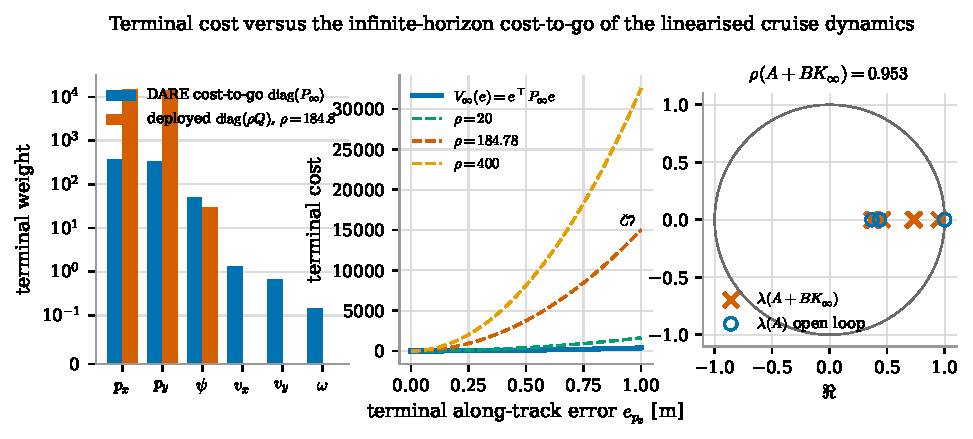
\includegraphics[width=\textwidth]{fig_lqr_terminal.pdf}
  \caption{Terminal cost versus the infinite-horizon cost-to-go of the linearised cruise dynamics. Left:
  diagonal of $P_\infty$ against the deployed $\rho Q$ (symmetric-log scale). Centre: terminal cost along a
  pure along-track error for $V_\infty$ and for three values of $\rho$. Right: open-loop eigenvalues of $A$
  and closed-loop eigenvalues of $A+BK_\infty$ in the unit disc.}
  \label{fig:lqrterminal}
\end{figure}

\subsubsection{Reference trajectory and warm start}
\label{sec:refwarm}

The reference $\{x_{\mathrm{ref},k}\}_{k=0}^{N}$ is obtained by advancing along the smoothed \astar{} path at
the cruise speed $v_{\mathrm{ref}}=0.5$~m/s from the arc-length coordinate $s_0$ of the path point closest to
the robot,
\begin{equation}
  s_k=\min\!\left(s_0+v_{\mathrm{ref}}\,k\,\Delta t,\; L_{\mathrm{path}}\right),
  \label{eq:ref}
\end{equation}
linearly interpolating the position inside the containing segment and taking the heading as the segment
tangent, $\psi_{\mathrm{ref},k}=\mathrm{atan2}(\Delta y,\Delta x)$. When the path is shorter than
$v_{\mathrm{ref}}N\Delta t$ the reference saturates at its end point, which turns the tracking term into a
terminal-position term --- the mechanism by which the controller decelerates into the local goal.

The previous solution is reused as the initial guess by the standard shift-and-append rule
\begin{equation}
  U^{(0)}_{\text{new}} = \big[u^\star_1,\dots,u^\star_{N-1},u^\star_{N-1}\big],\qquad
  X^{(0)}_{\text{new}} = \big[x^\star_1,\dots,x^\star_{N},x^\star_{N}\big],
  \label{eq:warm}
\end{equation}
which is consistent to first order because the reference itself shifts by one step. Two safeguards protect
the warm start: it is discarded whenever IPOPT reports a failure, and it is discarded when the optimal cost
exceeds five times the mean of the last seven solves. The second rule matters because a cost spike signals
that the reference topology has jumped (a new wall entered the window, the \astar{} path switched homotopy
class), in which case the shifted guess lies in the basin of the \emph{old} solution and would slow the solver
down or drag it to a poor local minimum. Section~\ref{sec:warmstart} quantifies the benefit of the warm start
at $38.7\%$ of the computation time.

\subsubsection{On the absence of integral action}
\label{sec:integral}

The formulation has no integral action and no disturbance estimator: the state~\eqref{eq:state} is not
augmented with an input-disturbance model, and the reference~\eqref{eq:ref} is tracked in a purely
proportional--predictive sense. For a nominal plant this is immaterial, but any constant unmodelled input ---
a mis-identified $\tau$, a lateral drift of the gait, a slope --- produces a persistent offset from the path
rather than being integrated away. Section~\ref{sec:mismatch} measures that offset; Section~\ref{sec:discussion}
discusses the standard remedy (state augmentation with an integrated tracking error, as in the
velocity-form MPC of \cite{rawlings2017mpc}).

%=============================================================================
\section{Optimization procedure}
\label{sec:optproc}

\subsection{Problem dimensions and structure}
\label{sec:dims}

Table~\ref{tab:nlp} reports the size of the NLP at the deployed setting $N=50$, $M=12$. It is a
medium-scale, sparse, smooth, non-convex problem: $456$ decision variables, $306$ equality constraints,
$300$ simple bounds and $1224$ barrier terms in the objective. The Jacobian of~\eqref{eq:cons-dyn} is block
bi-diagonal, with $6\times9$ blocks coupling $(x_k,u_k)$ to $x_{k+1}$; the Hessian of the Lagrangian is block
tri-diagonal, the off-diagonal input blocks coming from the rate penalty. Nothing in the problem couples
distant stages, so the linear algebra cost of an interior-point iteration is linear in $N$ --- a prediction
confirmed to within a few percent by the measured $0.52$~ms per additional horizon step
(Section~\ref{sec:horizon}).

\begin{table}[htbp]
  \centering
  \small
  \caption{NLP dimensions at the deployed configuration $N=50$, $\Delta t=0.1$~s, $M=12$.}
  \label{tab:nlp}
  \begin{tabular}{llr}
    \toprule
    Quantity & Expression & Value \\
    \midrule
    State variables            & $6(N+1)$        & $306$ \\
    Input variables            & $3N$            & $150$ \\
    Total decision variables   & $6(N+1)+3N$     & $\mathbf{456}$ \\
    Dynamic equalities         & $6N$            & $300$ \\
    Initial-state equalities   & $6$             & $6$ \\
    Input bounds               & $6N$            & $300$ \\
    Barrier terms (sigmoid + quadratic) & $2M(N+1)$ & $1224$ \\
    Nonlinear elementary functions per solve & $2(N+1)M+2N$ & $1324$ \\
    \bottomrule
  \end{tabular}
\end{table}

\subsection{Solver methodology}
\label{sec:solver}

The NLP is solved with IPOPT \cite{wachter2006ipopt}, a primal--dual interior-point method with a filter
line-search. Writing the problem as $\min_z \phi(z)$ s.t.\ $c(z)=0$, $z^L\le z\le z^U$, IPOPT replaces the
bounds with a logarithmic barrier
\begin{equation}
  \varphi_\mu(z) \;=\; \phi(z) \;-\; \mu\sum_i\Big[\ln\!\big(z_i-z_i^L\big)+\ln\!\big(z_i^U-z_i\big)\Big],
  \label{eq:ipopt}
\end{equation}
solves the resulting equality-constrained problem approximately by a Newton step on the perturbed
Karush--Kuhn--Tucker system, and drives the barrier parameter $\mu\to0$. Each iteration requires one
factorisation of the sparse symmetric indefinite KKT matrix
\begin{equation}
  \begin{bmatrix}
    \nabla^2_{zz}\mathcal{L} + \Sigma & \nabla c(z)^{\!\top}\\
    \nabla c(z) & 0
  \end{bmatrix}
  \begin{bmatrix}\Delta z\\ \Delta\lambda\end{bmatrix}
  = -\begin{bmatrix}\nabla\varphi_\mu\\ c(z)\end{bmatrix},
  \label{eq:kkt}
\end{equation}
with $\Sigma$ the diagonal barrier contribution, performed by MUMPS on the sparsity pattern described above.
The choice fits this problem for three reasons: the constraint set is dominated by equalities, for which
interior-point methods are far more efficient than active-set methods (there is no combinatorial active-set
identification to perform, only $300$ simple bounds); exact first and second derivatives are available
analytically from CasADi's algorithmic differentiation, so the full Newton system~\eqref{eq:kkt} can be used
rather than a quasi-Newton approximation; and the filter line-search copes with the strongly nonconvex
barrier landscape of~\eqref{eq:barrier} without requiring a globally convex model.

The known weakness of an interior-point method in a real-time loop is that it cannot be warm-started as
effectively as an active-set or a real-time-iteration scheme \cite{diehl2005realtime}: the barrier
parameter must be re-initialised and the iterates must be pushed strictly inside the bounds, which discards
part of the information in~\eqref{eq:warm}. This is visible in Section~\ref{sec:warmstart}, where the warm
start saves $38.7\%$ of the computation but not the order of magnitude one would obtain from a properly
warm-started sequential quadratic program.

\subsection{Implementation and configuration}
\label{sec:impl}

The program is built once, symbolically, with the CasADi \texttt{Opti} interface, and every quantity that
changes between cycles is a \emph{parameter} rather than a constant:
\begin{itemize}\itemsep2pt
  \item $\hat x\in\R^{6}$, the measured initial state;
  \item $X_{\mathrm{ref}}\in\R^{6\times(N+1)}$, the reference from~\eqref{eq:ref};
  \item $\mathcal{O}\in\R^{2\times M}$, the (sentinel-padded) obstacle positions;
  \item the three velocity bounds of~\eqref{eq:cons-vx}--\eqref{eq:cons-vyw}.
\end{itemize}
Consequently the expression graph, the derivative code and the sparsity patterns are generated exactly once at
start-up; a cycle only writes numbers into parameter slots and calls the solver. The graph is flattened with
\texttt{expand:\,true}, which converts the \texttt{MX} graph into scalar \texttt{SX} operations and removes
the interpreter overhead that would otherwise dominate a problem with $1324$ elementary nonlinear
operations. The first solve after start-up therefore pays a one-off construction and code-generation cost of
$0.35$--$1.0$~s depending on $N$ (Section~\ref{sec:horizon}); this is the single deadline violation of the
entire run, and the deployment absorbs it by holding the robot still during initialisation.

Solver options are deliberately austere: \texttt{max\_iter}$=100$, \texttt{print\_level}$=0$,
\texttt{warm\_start\_init\_point} enabled. No CPU-time limit is imposed inside IPOPT; the real-time
protection lives in the supervisor instead, which is the more robust arrangement because it keeps the solver
deterministic. That supervisor implements three mechanisms, all of which are part of the deployed
configuration and all of which exist because a $10$~Hz loop cannot afford to wait for a perfect solution:
\begin{enumerate}[label=\arabic*.]
  \item \textbf{Warm-start hygiene} --- the cache is cleared on solver failure and on a cost spike
        (Section~\ref{sec:refwarm}).
  \item \textbf{Zero-velocity fallback} --- after three consecutive IPOPT failures the tracker stops
        publishing optimised commands and returns a zero input, which is always feasible and always safe;
        this is preferable to applying the last usable solution, which is by then stale.
  \item \textbf{Adaptive input bounds} --- when the observed failure rate exceeds $30\%$ the supervisor
        shrinks $v_{x,\max}$ through the parameter interface, reducing the distance the horizon covers and
        thereby the number of active barrier terms, and restores it when the failure rate drops below $5\%$.
\end{enumerate}
In all the closed-loop campaigns reported in Section~\ref{sec:performance} the solver never failed
($n_{\mathrm{fail}}=0$ over more than $20\,000$ solves), so mechanisms~2 and~3 were never triggered; they are
documented because they are what makes the deployment survive on hardware, where a stale LiDAR frame or an EKF
jump can produce an ill-posed instance.

\subsection{Offline weight tuning by per-axis Gaussian processes}
\label{sec:bo}

\subsubsection{The tuning problem}

The eleven weights
\begin{equation}
  \theta=\big(Q_x,\,Q_y,\,Q_\psi,\,\rho,\,R_{v_x},\,R_{v_y},\,R_\omega,\,\Rjerk,\,\Wobs,\,\aobs,\,\robs\big)\in\Theta\subset\R^{11}
  \label{eq:theta}
\end{equation}
are the design variables of a second-level problem
\begin{equation}
  \hat\theta \;=\; \arg\min_{\theta\in\Theta} \mathcal{J}(\theta),
  \label{eq:outer}
\end{equation}
where $\mathcal{J}$ measures closed-loop navigation quality. Problem~\eqref{eq:outer} shares none of the
structure of the inner NLP: $\mathcal{J}$ has no closed form, no derivatives, and a single evaluation costs a
full navigation rollout. It is a black-box problem, and the natural tool is a Gaussian-process surrogate
\cite{rasmussen2006gp,shahriari2016bo}.

The obstacle is dimension. A surrogate over $\Theta\subset\R^{11}$ needs a sample density that a rollout-priced
objective cannot supply: a budget of $n$ evaluations covers each axis with only $n^{1/11}$ points, so even a
hundred rollouts amount to fewer than two points per coordinate. A surrogate fitted on such a sample spends
most of its capacity on coordinates that turn out not to matter, and any acquisition rule that rewards
unexplored regions never runs out of them.

\subsubsection{Objective}

Each evaluation is a full closed-loop mission in the pillar-field world $\mathrm{E}_c$
(Section~\ref{sec:setup}), driving the production tracker with a $40$~s cap:
\begin{equation}
  \mathcal{J}_{\mathrm{cl}}(\theta)=
  \begin{cases}
    T_{\mathrm{goal}}/T_{\mathrm{ref}}, & \text{goal reached},\\[2pt]
    10+5\,d_{\mathrm{final}}/d_0, & \text{otherwise},
  \end{cases}
  \;+\;0.5\,\overline{\|\Delta u\|}\;+\;0.01\,\bar t\;+\;2\max(0,\,0.25-d_{\min}),
  \label{eq:Jcl}
\end{equation}
with $T_{\mathrm{ref}}=d_0/v_{\mathrm{ref}}$ the time a straight run at cruise speed would take,
$d_{\mathrm{final}}$ the residual distance to the goal, $\overline{\|\Delta u\|}$ the mean input increment,
$\bar t$ the mean solve time in milliseconds and $d_{\min}$ the minimum clearance. The branch structure is
deliberate: a configuration that does not complete the mission is scored on the fraction of the distance it
closed, which keeps the objective informative on failures instead of saturating at a constant penalty. The
four additive terms then rank the successful configurations by time, smoothness, computational cost and
safety margin, in that order of magnitude. Unlike a one-step prediction score evaluated on a recorded
trajectory, \eqref{eq:Jcl} can observe a deadlock --- which, as Section~\ref{sec:barriersweep} shows, is
precisely the failure the barrier weights are capable of producing.

\subsubsection{Per-axis surrogates and coordinate descent}

Rather than one surrogate over $\R^{11}$, the scheme fits \emph{eleven one-dimensional} Gaussian processes,
one per coordinate. Writing $\theta=(\theta_i,\theta_{-i})$, each axis is explored on a uniform design of
$m=6$ values spanning its interval while $\theta_{-i}$ is held fixed, and a $1$-D GP with a Mat\'ern-$5/2$
kernel and a white-noise term,
\begin{equation}
  k(\theta_i,\theta_i')=\sigma_f^2\Big(1+\sqrt5\,\tfrac{|\theta_i-\theta_i'|}{\ell}
  +\tfrac53\tfrac{(\theta_i-\theta_i')^2}{\ell^2}\Big)e^{-\sqrt5|\theta_i-\theta_i'|/\ell}
  +\sigma_n^2\delta(\theta_i,\theta_i'),
  \label{eq:kernel}
\end{equation}
is fitted to the six observations by maximising the log marginal likelihood. The axis optimum is the
minimiser of the posterior mean over a fine grid,
\begin{equation}
  \hat\theta_i \;=\; \arg\min_{\theta_i\in[\ell_i,u_i]}\; \mu_i(\theta_i),
  \label{eq:axisopt}
\end{equation}
which uses the smoothed estimate rather than the best sampled point and therefore does not require the
optimum to coincide with a grid node.

Three design decisions make the scheme work, and each is validated in Section~\ref{sec:ofat}.

\paragraph{Separability.} Assembling per-axis optima into a single vector is exact when the objective is
additively separable, $\mathcal{J}(\theta)\approx\sum_i f_i(\theta_i)$. That assumption is not exactly true
here --- the barrier height and the safety radius interact, since a tall barrier is harmless when its radius
is small (Section~\ref{sec:barriersweep}) --- so it is not relied upon blindly, but repaired by the next
decision and verified a posteriori by evaluating the assembled vector.

\paragraph{Sequential update and ordering.} The axes are swept in decreasing order of influence and each
optimum is \emph{fixed before the next axis is visited}, so that later sweeps are conducted about an already
improved operating point. This is coordinate descent with a GP line search, and it is what makes the scheme
robust to the interactions that separability ignores: sweeping the dominant coordinate first moves the base
point out of the deadlocked region, so that every subsequent sweep is measured where the objective actually
discriminates. Section~\ref{sec:ofat} quantifies the difference against the naive arrangement.

\paragraph{Significance floor.} A $1$-D GP fitted to six points will return an optimum on any axis, including
one on which the objective does not move. An axis is therefore accepted only if the spread of its six
observations, $\Delta\mathcal{J}_i$, exceeds the run-to-run scatter; otherwise the weight keeps its default.
The last column of Table~\ref{tab:params} reports that spread, and the criterion retains five of the eleven
weights.

The total cost is $11m+1=67$ evaluations, and every one of them is a mission-level rollout rather than a
proxy. The by-product is as valuable as the optimum: eleven curves with error bands, each showing how much
the objective actually depends on the weight in question, on which the reader can check the tuning rather
than trust it.

\begin{table}[htbp]
  \centering
  \small
  \caption{The eleven tuned weights: hand-tuned baseline $\thn$, the interval swept by the per-axis scheme,
  the resulting optimum $\hat\theta$, and the spread $\Delta\mathcal{J}_i$ of the six observations on that
  axis. Weights whose spread falls below the significance floor (grey) are not identified by the data and keep
  their default. The last column is the vector currently shipped in the repository's
  \texttt{planner\_params.yaml}, used as the reference configuration in Section~\ref{sec:performance}.}
  \label{tab:params}
  \setlength{\tabcolsep}{5pt}
  \begin{tabular}{llrlrrr}
    \toprule
    Symbol & Meaning & $\thn$ & swept interval & $\hat\theta$ & $\Delta\mathcal{J}_i$ & deployed \\
    \midrule
    $\robs$    & safety radius [m]            & $0.8$   & $[0.05,\,1]$  & $0.098$  & $\mathbf{13.01}$ & $0.098$ \\
    $\aobs$    & barrier steepness [m$^{-1}$] & $8.0$   & $[0.1,\,15]$  & $12.06$  & $\mathbf{13.75}$ & $13.44$ \\
    $R_{v_x}$  & forward effort               & $1.0$   & $[0.1,\,10]$  & $9.74$   & $0.107$ & $9.95$ \\
    $\Wobs$    & barrier height               & $500.0$ & $[1,\,500]$   & $167.9$  & $0.077$ & $4.83$ \\
    $R_{v_y}$  & lateral effort               & $1.0$   & $[0.1,\,10]$  & $10.0$   & $0.074$ & $8.11$ \\
    \midrule
    \rowcolor{black!6} $Q_\psi$   & heading weight    & $0.5$   & $[0,\,15]$   & $0.75$  & $0.044$ & $0.160$ \\
    \rowcolor{black!6} $Q_x$      & along-track weight& $20.0$  & $[50,\,200]$ & $50.0$  & $0.039$ & $81.41$ \\
    \rowcolor{black!6} $Q_y$      & cross-track weight& $20.0$  & $[50,\,200]$ & $50.0$  & $0.023$ & $76.79$ \\
    \rowcolor{black!6} $\Rjerk$   & input-rate penalty& $0.2$   & $[0.1,\,5]$  & $5.0$   & $0.017$ & $2.68$ \\
    \rowcolor{black!6} $R_\omega$ & yaw-rate effort   & $0.5$   & $[0.1,\,10]$ & $5.89$  & $0.007$ & $9.81$ \\
    \rowcolor{black!6} $\rho$     & terminal multiplier& $50.0$ & $[50,\,300]$ & $198.0$ & $0.004$ & $184.78$ \\
    \bottomrule
  \end{tabular}
\end{table}

Table~\ref{tab:params} already tells the story that the rest of the report confirms. The two axes that clear
the significance floor by three orders of magnitude are both barrier parameters, and the tuning moves them in
a consistent direction: it makes the barrier \emph{narrow} ($\robs$ from $0.80$ to $0.098$~m) and
\emph{steep} ($\aobs$ from $8$ to $12.1$~m$^{-1}$), demoting~\eqref{eq:barrier} from a long-range repulsive
field to a short-range safety net and delegating geometric obstacle avoidance to the \astar{} layer that is
already solving that problem globally on the grid. One number in this story must not be taken at face
value: $\robs=0.098$~m is the optimum for a robot \emph{with no body}. The harness plant is a point, so the
tuner is free to strip the safety net down to almost nothing and cash the freed clearance in as progress;
on the physical platform the same number places the barrier boundary well inside the robot's own footprint,
and the quadruped brushes every door frame it passes. The deployed configuration therefore floors the
safety radius at the body radius, $\robs\ge0.30$~m --- the direction of the tuning result (narrow and
steep) is kept, its magnitude is bounded below by the geometry the tuning objective could not see.
Section~\ref{sec:memoryfix} returns to this point when the stack runs on the simulated quadruped. The
effort weights rise by an order of magnitude, which buys smoothness. The six greyed weights --- among them every tracking weight and the terminal multiplier ---
do not move the objective measurably, and the report's parametric studies in Sections~\ref{sec:weights}
and~\ref{sec:terminalsweep} confirm independently that they are weak knobs.

%=============================================================================
\section{Performance analysis}
\label{sec:performance}

\subsection{Experimental setup}
\label{sec:setup}

All results in this section come from an offline closed-loop harness that imports the \emph{production}
modules --- \texttt{FixedGaussianGridMap}, \texttt{AStarPlanner}, \texttt{MPCTracker} --- so every reported
number is generated by the deployed formulation and the deployed solver, not by a re-implementation. Two
deliberate simplifications isolate the optimization layer from the rest of the stack:
\begin{itemize}
  \item the ROS~2 cascade (setpoint low-pass filter and proportional \texttt{/cmd\_vel} controller) is
        bypassed and $u^\star_0$ is applied directly to the plant, which is the textbook receding-horizon
        implementation;
  \item obstacle memory is switchable. With the persistent cell map \emph{disabled} the planner sees only
        the current scan --- the worst case for the rolling-horizon rule~\eqref{eq:localgoal}, and what
        makes the failure mode of Section~\ref{sec:localmin} observable. Section~\ref{sec:memoryfix}
        switches the memory on, re-poses the target rule on it, and shows that this closes the failure.
\end{itemize}
The plant is the discrete model~\eqref{eq:veldisc}--\eqref{eq:posedisc}; the sensor is a ray-marched $180$-beam
planar LiDAR with $6$~m range and $\sigma_{\mathrm{noise}}=1$~cm. Replanning runs at $1$~Hz, control at
$1/\Delta t$. Three worlds are used (Fig.~\ref{fig:closedloop}):

\begin{itemize}
  \item $\mathrm{E}_a$ --- \textbf{two-room office}, $16\times11$~m, two partitions with narrow doorways and
        scattered furniture; the goal lies two rooms away, so the rolling-horizon rule is stressed;
  \item $\mathrm{E}_b$ --- \textbf{S-corridor}, $14\times8$~m, three staggered partitions forming a
        serpentine of ${\sim}2.5$~m width; a stress test for barrier conditioning;
  \item $\mathrm{E}_c$ --- \textbf{pillar field}, $14\times10$~m, $16$ randomly placed boxes; the
        obstacle-dense case used for the weight sweeps.
\end{itemize}

Reported metrics are: success (goal reached within $0.45$~m before the time cap), time to goal (TTG),
distance travelled, mean/95th-percentile/maximum solve time, mean IPOPT iterations, RMS and maximum distance
to the \astar{} reference, minimum true clearance to an obstacle, and mean input increment
$\overline{\|\Delta u\|}$ as a smoothness proxy. All timings were measured single-threaded on an Intel Core
i7-13650HX with CasADi $3.7.2$ and IPOPT/MUMPS; the on-robot computer is a Jetson Orin Nano, roughly
$3$--$4\times$ slower, which is the factor to keep in mind when reading the $100$~ms deadline lines in the
figures.

\subsection{Baseline versus tuned weights in closed loop}
\label{sec:closedloop}

Table~\ref{tab:closedloop} and Fig.~\ref{fig:closedloop} compare the hand-tuned baseline $\thn$ with the
configuration $\thst$ currently deployed on the robot, under otherwise identical conditions ($N=50$, $\Delta t=0.1$~s, $M=12$, $120$~s
cap).

\begin{table}[htbp]
  \centering
  \small
  \caption{Closed-loop comparison of the hand-tuned baseline $\thn$ and the deployed $\thst$. TTG is the
  elapsed time, capped at $120$~s; ``dist.'' is the distance actually travelled, so a large value with
  ``no'' in the success column indicates wandering rather than progress. $\bar t$ and $t_{95}$ are the mean
  and $95$th-percentile solve times, $\bar\nu$ the mean IPOPT iteration count, $e_{\mathrm{rms}}$ the RMS
  distance to the \astar{} reference, $d_{\min}$ the minimum true clearance.}
  \label{tab:closedloop}
  \begin{tabular}{llccrrrrrrr}
    \toprule
    World & $\theta$ & goal & TTG [s] & dist.\ [m] & $\bar t$ [ms] & $t_{95}$ [ms] & $\bar\nu$ &
    $e_{\mathrm{rms}}$ [m] & $d_{\min}$ [m] & $\overline{\|\Delta u\|}$ \\
    \midrule
    \multirow{2}{*}{$\mathrm{E}_a$ office}
      & $\thn$  & no  & $>120$ & $8.06$  & $55.8$ & $62.7$ & $16.0$ & $0.061$ & $0.99$ & $0.085$ \\
      & $\thst$ & no  & $>120$ & $52.91$ & $37.9$ & $65.6$ & $11.3$ & $0.047$ & $0.31$ & $0.163$ \\
    \midrule
    \multirow{2}{*}{$\mathrm{E}_b$ corridor}
      & $\thn$  & no  & $>120$ & $8.01$  & $41.6$ & $51.4$ & $11.7$ & $0.041$ & $1.05$ & $0.123$ \\
      & $\thst$ & \textbf{yes} & $\mathbf{33.9}$ & $16.74$ & $29.1$ & $47.2$ & $7.7$ & $0.046$ & $0.30$ & $0.166$ \\
    \midrule
    \multirow{2}{*}{$\mathrm{E}_c$ clutter}
      & $\thn$  & no  & $>120$ & $6.99$  & $55.8$ & $63.8$ & $16.5$ & $0.013$ & $1.05$ & $0.126$ \\
      & $\thst$ & \textbf{yes} & $\mathbf{27.9}$ & $13.55$ & $30.2$ & $52.8$ & $6.9$ & $0.047$ & $0.65$ & $0.173$ \\
    \bottomrule
  \end{tabular}
\end{table}

\begin{figure}[htbp]
  \centering
  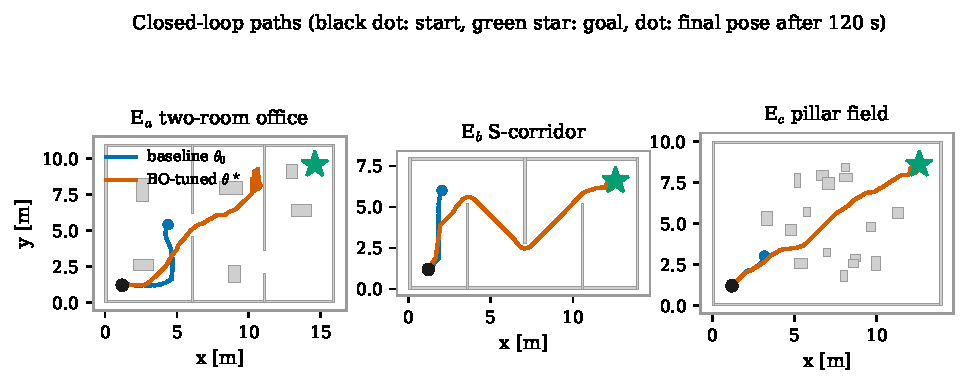
\includegraphics[width=\textwidth]{fig_closed_loop.pdf}
  \caption{Executed paths in the three worlds for the baseline (blue) and the deployed weights (orange);
  black dot is the start, green star the goal, filled circles the final pose. The baseline stalls a few
  metres from the start in all three worlds; the tuned controller reaches the goal in
  $\mathrm{E}_b$ and $\mathrm{E}_c$ and wanders in $\mathrm{E}_a$ (Section~\ref{sec:localmin}).}
  \label{fig:closedloop}
\end{figure}

The difference is not quantitative but qualitative: the baseline \emph{never reaches the goal}, in any world.
It travels $7$--$8$~m in $120$~s and its minimum clearance is exactly its initial clearance
($1.05$~m in $\mathrm{E}_b$ and $\mathrm{E}_c$), i.e.\ it never approaches anything. The mechanism is visible
in Table~\ref{tab:params}: with $\Wobs=500$ and $\robs=0.8$~m, the barrier contributes up to
$\Wobs M=6000$ cost units per node against a tracking term of order $Q_x e^2\approx20$ for a decimetre of
error. The optimizer's cost function is dominated by a repulsive field that extends about a metre from every
LiDAR return, and in a corridor of finite width the cheapest predicted trajectory is to stop. This is not a
tuning subtlety --- it is the barrier-weight failure reproduced deliberately and independently in
Section~\ref{sec:barriersweep}, where any $\Wobs\ge50$ freezes the robot.

Where the tuned controller does complete the mission it is also cheaper and better conditioned: $-30\%$ mean
solve time ($41.6\to29.1$~ms in $\mathrm{E}_b$, $55.8\to30.2$~ms in $\mathrm{E}_c$) and $-34$ to $-58\%$
IPOPT iterations, because a weak, narrow barrier produces a far flatter objective landscape than a heavy,
wide one. Tracking accuracy is comparable ($e_{\mathrm{rms}}\approx4.6$~cm), and smoothness is
\emph{worse} ($\overline{\|\Delta u\|}$ $0.12\to0.17$) --- unsurprising, since the tuned controller is
actually manoeuvring at $0.5$~m/s while the baseline is nearly stationary.

\subsection{The rolling-horizon local minimum}
\label{sec:localmin}

In the office world $\mathrm{E}_a$ the tuned controller travels $52.9$~m in $120$~s without reaching a goal
that is $16$~m away. Fig.~\ref{fig:localmin} shows why. The local target follows the ray to the global goal
into the partition wall; \astar{} correctly routes around the obstacle \emph{inside the window}, the MPC
tracks that path faithfully ($e_{\mathrm{rms}}=4.7$~cm), and one grid width later the same rule sends the
robot back --- with the memory of the wall already erased, since the grid is rebuilt from the current scan
only. The result is a limit cycle: locally optimal at every cycle, globally useless.

\begin{figure}[htbp]
  \centering
  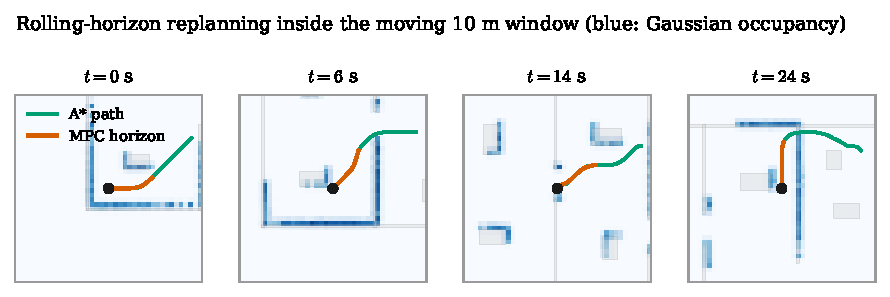
\includegraphics[width=\textwidth]{fig_local_minimum.pdf}
  \caption{Four snapshots of a rolling-horizon cycle in $\mathrm{E}_a$ (blue field: Gaussian occupancy in the
  moving $10\times10$~m window; green: \astar{} path; orange: MPC prediction). The optimization is solved
  correctly at every cycle --- the failure is in the greedy target rule~\eqref{eq:localgoal}, not in the NLP.}
  \label{fig:localmin}
\end{figure}

Three structural facts conspire here, and all three are properties of the \emph{formulation} rather than of
the solver: the target rule~\eqref{eq:localgoal} is memoryless; the occupancy grid is volatile; and
constraint~\eqref{eq:cons-vx} forbids reversing, so the only escape from a concave pocket is a wide forward
arc. Adding memory is therefore not a refinement but a requirement. Section~\ref{sec:memoryfix} adds it ---
the persistent cell map is switched on and the target rule is re-posed as a shortest-path problem on the
remembered world --- and the same trap is then solved. This is the clearest illustration in the whole study
of the difference between solving an optimization problem well and posing the right one.

\subsection{Closing the limit cycle: a memory-augmented target rule}
\label{sec:memoryfix}

The failure of Fig.~\ref{fig:localmin} lives in the target rule, so the repair must live there too. This
subsection re-poses~\eqref{eq:localgoal} on an obstacle \emph{memory}, states the two design decisions that
make the re-posed rule sound, and validates it --- first in the harness, then in a full physics simulation
of the same world. The experiments run in a re-instantiation of the harness of Section~\ref{sec:setup} (the
three worlds rebuilt from their specification, every module still the production code), in which the
memoryless configuration reproduces the failure of Section~\ref{sec:localmin} exactly: $50.4$~m travelled in
$120$~s, goal never reached, the trap now a clean period-$10$~s limit cycle of $0.4$~m amplitude against the
second partition (Fig.~\ref{fig:memoryfix}, left).

\paragraph{Memory.} Every LiDAR return is quantised to its $\Delta$-cell in the \emph{world} frame and
stored with two scalars: the time it was last seen and the number of \emph{distinct scans} in which it has
appeared. A cell is \emph{confirmed} once that count reaches two; unconfirmed cells expire with the map's
decay time. This one-line filter is what keeps the memory honest against sensor noise: a wall is re-hit by
every scan that ranges it, while a spurious return lands in its cell exactly once and is never allowed to
become an obstacle. Confirmation lets evidence accumulate; a second mechanism lets contradicting evidence
win: every beam that passes \emph{through} a remembered cell on its way to a farther return deletes that
cell (free-space carving, stopping half a metre short of the endpoint so a ray never carves the surface it
terminates on). A real wall cannot be carved --- beams end on it --- while a phantom cell standing in an
open passage is crossed, and erased, by every scan that ranges through the passage. In the static harness
with exact localisation carving is essentially inert and the decay is disabled; both mechanisms earn their
place in the physics validation below, and the deployed stack keeps its $20$~s decay so that moving
obstacles are eventually forgotten. Only confirmed cells are allowed to touch the planner at all --- hard
vetoes and soft inflation alike --- so a one-off return never perturbs a cost anywhere.

\paragraph{The global grid, and two hardening rules.} Let $\mathcal{M}_k$ be the confirmed cells at cycle
$k$. A global grid $\mathcal{G}_k$ is built over the bounding box of $\mathcal{M}_k\cup\{\hat x,x_g\}$ with
the same resolution and the same Gaussian inflation~\eqref{eq:grid} as the local window, evaluated against
the remembered cells; space never observed is optimistically free. Three further rules are essential, and
each was found by watching its absence fail. First, \textbf{confirmed cells are removed from the search
graph outright} --- from the global grid \emph{and} from the local window --- not merely inflated. The tail
of~\eqref{eq:grid} hard-blocks only cells within $0.25\sigma\approx4$~cm of a return, so under the soft
cost~\eqref{eq:astarcost} a remembered wall is a \emph{finite} obstacle --- crossing it costs the search
roughly $(1+w_{\mathrm{obs}})\Delta\approx9$~m of equivalent path length --- and an early version of this
rule dutifully tunnelled through the partition of $\mathrm{E}_a$ the moment the true detour ($\approx14$~m)
became more expensive than the wall. Inflation prices \emph{proximity}; memory records \emph{evidence}; only
the latter may veto an edge, and it must veto it in both graphs, because a target that is legal globally can
still tempt the \emph{local} search through a soft wall when goal and detour both fit in the window. Second,
\textbf{one-cell pinholes among confirmed cells are sealed in the routing graph}: at the sensor's $6$~m
range the $2°$ beam spacing exceeds the $0.25$~m cell size, so a remembered wall carries single-cell gaps
that open and close as scans accumulate --- each one a phantom shortcut that flips the global route and,
before sealing, left the robot dithering between the two ends of a half-confirmed wall. A gap narrower than
one cell is narrower than the robot; it is never a route. Third, \textbf{the local execution graph carries
the body}: confirmed cells are dilated by the robot radius ($0.25$~m) before they veto local edges, so no
executed path passes within a body radius of known structure --- a $4$~cm clearance, perfectly survivable
for the point mass of the harness, is a collision for a $0.37$~m-wide quadruped. The two graphs are
deliberately \emph{not} treated alike: dilating the routing graph as well makes the committed route
invalidate itself as the observed wall grows under the robot's own approach --- the rule falls back into
exploration --- while sealing the execution graph after dilation counts the body twice and closes every
doorway the robot actually fits through. Stability lives in the routing graph, clearance in the execution
graph, and the flooring of the MPC safety radius at the same body radius (the $\robs$ discussion of
Section~\ref{sec:bo}) closes the chain at the control layer.

\paragraph{The re-posed target rule.} With $\pi_k$ the \astar{} path from $\hat x$ to $x_g$ on
$\mathcal{G}_k$ (same edge cost~\eqref{eq:astarcost}), the local target becomes
\begin{equation}
  x_{\mathrm{local}} \;=\; \pi_k(s^\star),
  \qquad
  s^\star \;=\; \max\{\,s \;:\; \pi_k(s)\in\mathcal{W}(\hat x)\,\},
  \label{eq:memgoal}
\end{equation}
the point where the globally consistent route exits the local window $\mathcal{W}$; the local \astar{} of
Section~\ref{sec:astar} then refines the path inside the window, on the local grid augmented with the
remembered cells. Two remarks. First, \eqref{eq:memgoal} contains~\eqref{eq:localgoal} as its empty-memory
special case: with $\mathcal{M}_k=\varnothing$ the global grid is free space, $\pi_k$ is the straight
segment to the goal, and its window exit \emph{is} the ray--boundary intersection. The greedy rule is not
discarded; it is revealed as the prior from which evidence is allowed to subtract. Second, the rule
deliberately has no ``goal inside the window'' shortcut: containment is not reachability, and if the known
map forces a detour that leaves the window, the target must stay on the robot's side of the wall ---
handing the local planner a target beyond a remembered wall is precisely the invitation to tunnel that the
hard-cell rule exists to refuse. Third, the route is \emph{committed}: the previous $\pi_{k-1}$ is
re-anchored at the robot and re-costed on $\mathcal{G}_k$ at every cycle, and the fresh optimum replaces it
only when the committed route has become blocked or the new one undercuts it by more than $20\%$. While the
map is still filling in, rival routes differ by fractions of a cell cost, and a rule that swaps on
$\varepsilon$-improvements turns half-knowledge into oscillation. For the same reason the window-exit
point itself is \emph{held} until the route genuinely changes or the robot reaches it: under a churning
half-built map the exit point slides cycle to cycle, and the MPC otherwise chases a moving reference.

\paragraph{Why the limit cycle is structurally excluded.} In a static world $\mathcal{M}_k$ is monotone:
$\mathcal{M}_k\subseteq\mathcal{M}_{k+1}$, so the global graph only ever loses edges. Every attempt to use a
passage that turns out to be blocked adds the blocking cells to $\mathcal{M}_k$ and permanently deletes that
route; the grid is finite, so the rule can propose only finitely many distinct routes and can never propose
the same refuted one twice. This is the invariant the limit cycle of Section~\ref{sec:localmin} violated ---
there, the refutation was erased one grid width later --- and it is the same optimism-under-unknown argument
that underlies replanning algorithms of the D\textsuperscript{*} family \cite{koenig2005dstarlite}. The
price of optimism is, in general, a bounded exploration episode while unconfirmed gaps close; with scans
ingested at the sensor rate, pinholes sealed and the route committed, that episode collapses in
$\mathrm{E}_a$ to nothing visible --- the partition enters memory while the robot is still approaching it,
the global path flips to the doorway at first contact, and the descent begins without a single reversal
(Fig.~\ref{fig:memfixsnap}).

\begin{figure}[htbp]
  \centering
  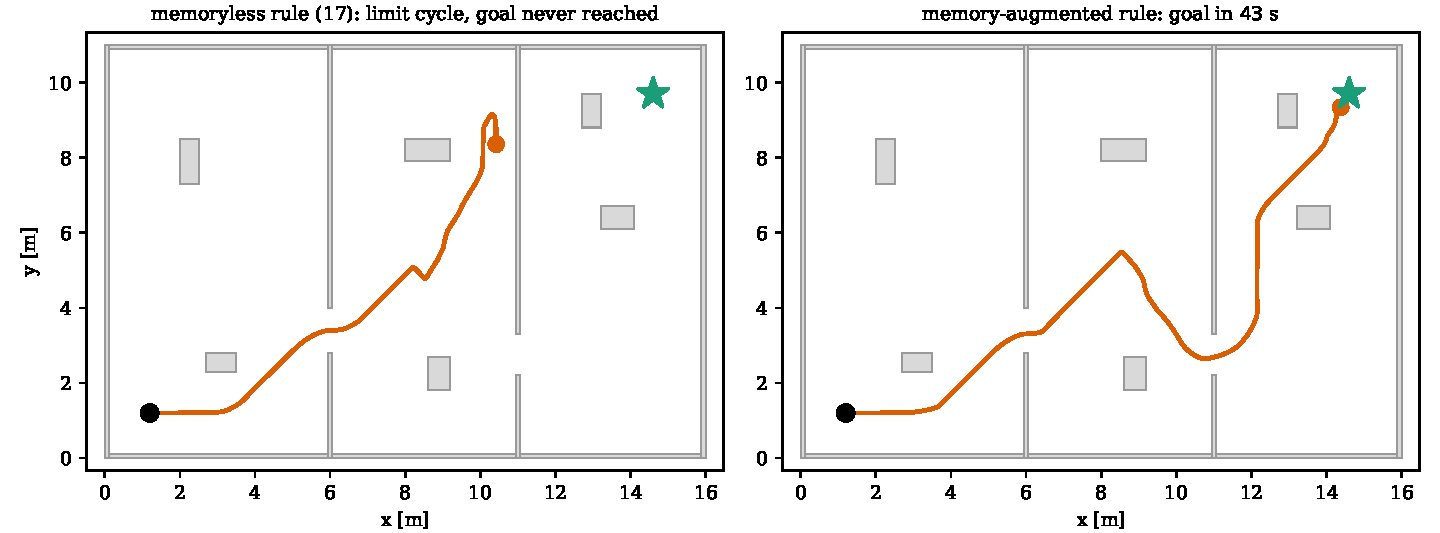
\includegraphics[width=\textwidth]{fig_memory_fix.pdf}
  \caption{The rebuilt $\mathrm{E}_a$ under the deployed weights $\thst$. Left: the memoryless
  rule~\eqref{eq:localgoal} locks into a period-$10$~s limit cycle at the second partition and never
  reaches the goal. Right: the memory-augmented rule~\eqref{eq:memgoal} turns down to the remembered doorway
  before ever reaching the wall and takes the goal in $43$~s. Same worlds, same NLP, same weights ---
  only the target rule differs.}
  \label{fig:memoryfix}
\end{figure}

\begin{figure}[htbp]
  \centering
  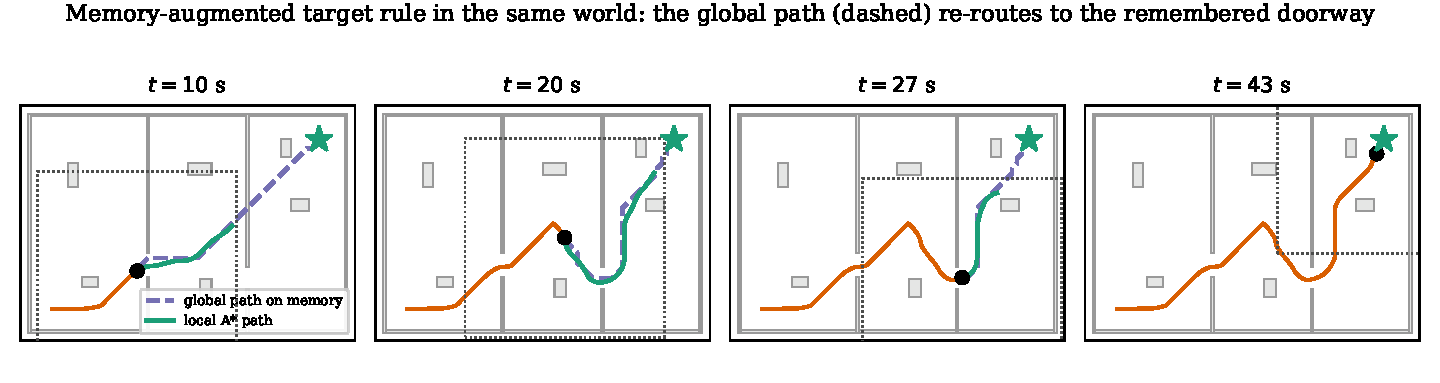
\includegraphics[width=\textwidth]{fig_local_minimum_fix.pdf}
  \caption{Four cycles of the memory-augmented rule in $\mathrm{E}_a$ (orange: executed trajectory; dashed:
  global path $\pi_k$ on the remembered map; green: local \astar{} path inside the dotted $10\times10$~m
  window). At $t=10$~s, crossing the first doorway, the second partition is not yet in memory and $\pi_k$
  is still the optimistic near-ray; by $t=20$~s the wall has been confirmed at a distance and the global
  path has flipped, once, to the doorway below --- the robot angles down before ever reaching the wall,
  threads the doorway at $t=27$~s and takes the goal at $t=43$~s without a single reversal.}
  \label{fig:memfixsnap}
\end{figure}

\begin{table}[htbp]
  \centering
  \small
  \caption{Memoryless rule~\eqref{eq:localgoal} against the memory-augmented rule~\eqref{eq:memgoal} in the
  rebuilt worlds, deployed weights $\thst$, $120$~s cap. The MPC layer is untouched by the change, so the
  solve-time statistics are those of Table~\ref{tab:closedloop}; the global layer adds $13$~ms per $1$~Hz
  replan on the fully mapped $\mathrm{E}_a$ ($371$ confirmed cells).}
  \label{tab:memoryfix}
  \begin{tabular}{llccccc}
    \toprule
    World & target rule & goal & TTG [s] & dist.\ [m] & $e_{\mathrm{rms}}$ [m] & $d_{\min}$ [m] \\
    \midrule
    \multirow{2}{*}{$\mathrm{E}_a$ office}
      & memoryless~\eqref{eq:localgoal} & no  & $>120$ & $50.35$ & $0.011$ & $0.51$ \\
      & memory~\eqref{eq:memgoal} & \textbf{yes} & $\mathbf{42.9}$ & $20.97$ & $0.016$ & $0.46$ \\
    \midrule
    \multirow{2}{*}{$\mathrm{E}_b$ corridor}
      & memoryless~\eqref{eq:localgoal} & \textbf{yes} & $\mathbf{36.9}$ & $18.06$ & $0.023$ & $0.31$ \\
      & memory~\eqref{eq:memgoal} & \textbf{yes} & $38.3$ & $18.45$ & $0.018$ & $0.42$ \\
    \midrule
    \multirow{2}{*}{$\mathrm{E}_c$ clutter}
      & memoryless~\eqref{eq:localgoal} & \textbf{yes} & $\mathbf{27.5}$ & $13.67$ & $0.021$ & $0.29$ \\
      & memory~\eqref{eq:memgoal} & \textbf{yes} & $29.2$ & $14.28$ & $0.015$ & $0.46$ \\
    \bottomrule
  \end{tabular}
\end{table}

Table~\ref{tab:memoryfix} is the quantitative summary. In $\mathrm{E}_a$ the rule converts a permanent
failure into a $42.9$~s success, and the comparison of distances is the cleanest possible statement of what
was wrong: the memoryless controller spends $50.4$~m of walking on a cycle, while the memory-augmented one
reaches a goal two rooms away in $21.0$~m --- well under half the distance the failing controller wastes,
and within two metres of the shortest route through the two doorways. In the two worlds that were already
solved the rule costs one to two seconds ($36.9\to38.3$~s, $27.5\to29.2$~s) and buys minimum clearance:
$0.31\to0.42$~m and $0.29\to0.46$~m --- the price of the body-radius dilation, paid where the memoryless
rule was shaving walls. In $\mathrm{E}_a$ the successful route holds $0.46$~m of clearance \emph{through}
the $1.1$~m doorway that the failing configuration never reached.

\paragraph{Validation in physics simulation.} As a final check that the mechanism, and not a property of
the point-mass harness, is what closes the failure, the same two-room world was rebuilt as a Gazebo
(Fortress) world and the \emph{complete} deployed stack was run on the simulated Go2 --- CHAMP gait
generator, EKF state estimation, the full ROS~2 cascade that the harness of Section~\ref{sec:setup}
deliberately bypasses, and the planner nodes importing the identical production modules. With the
memoryless rule the robot walks to the second partition and then slides along it for the remaining two
minutes --- it first touches the wall two body lengths from the doorway, and the ray rule walks it
\emph{away} from the door --- travelling $41$~m in $240$~s without reaching the goal. With the
memory-augmented rule (and the safety radius floored at the body radius) the robot walks the same route the
harness predicts: through the first doorway, down the second partition at first contact, through the lower
doorway and to the goal, in $142$~s of simulated time over $27.0$~m, without touching a wall. The gait
walks at roughly a third of the harness cruise speed, which accounts for the longer clock; the route and
its single commitment point are the same.

The full cascade also earned its place in the design: two of the memory mechanisms exist \emph{because} the
physics runs failed without them, and neither failure is observable in the harness, where localisation is
exact. State-estimation drift and the spin of the LiDAR smear wall returns across real openings; with
confirmation alone the phantom cells accumulate until the hardened map strangles the planner --- in one run
the remembered ``walls'' sealed the first doorway and boxed the robot into the starting room. Free-space
carving un-learns them, but carving \emph{without} the same-scan protection fails in the opposite
direction: the drifted rays pass through the true wall, erase it, and the robot spends the rest of the run
pushing against structure its map no longer contains. Confirmation, protected carving and the $30$~s decay
are jointly what keep a world-frame memory sane on top of a drifting estimator --- a genuinely
registration-limited regime that the clean harness cannot exhibit. Animated renderings of all runs, harness
and Gazebo, accompany this report in \texttt{Videos/}.

\subsection{Weight tuning by per-axis Gaussian processes}
\label{sec:ofat}

Fig.~\ref{fig:ofatcurves} is the complete output of the tuning procedure of Section~\ref{sec:bo}: for each of
the eleven weights, six real closed-loop evaluations and the one-dimensional Gaussian process fitted to them.
Because every other coordinate is genuinely held fixed while an axis is swept, the plotted observations lie on
the plotted curve --- a property no slice through a joint surrogate can claim.

\begin{figure}[htbp]
  \centering
  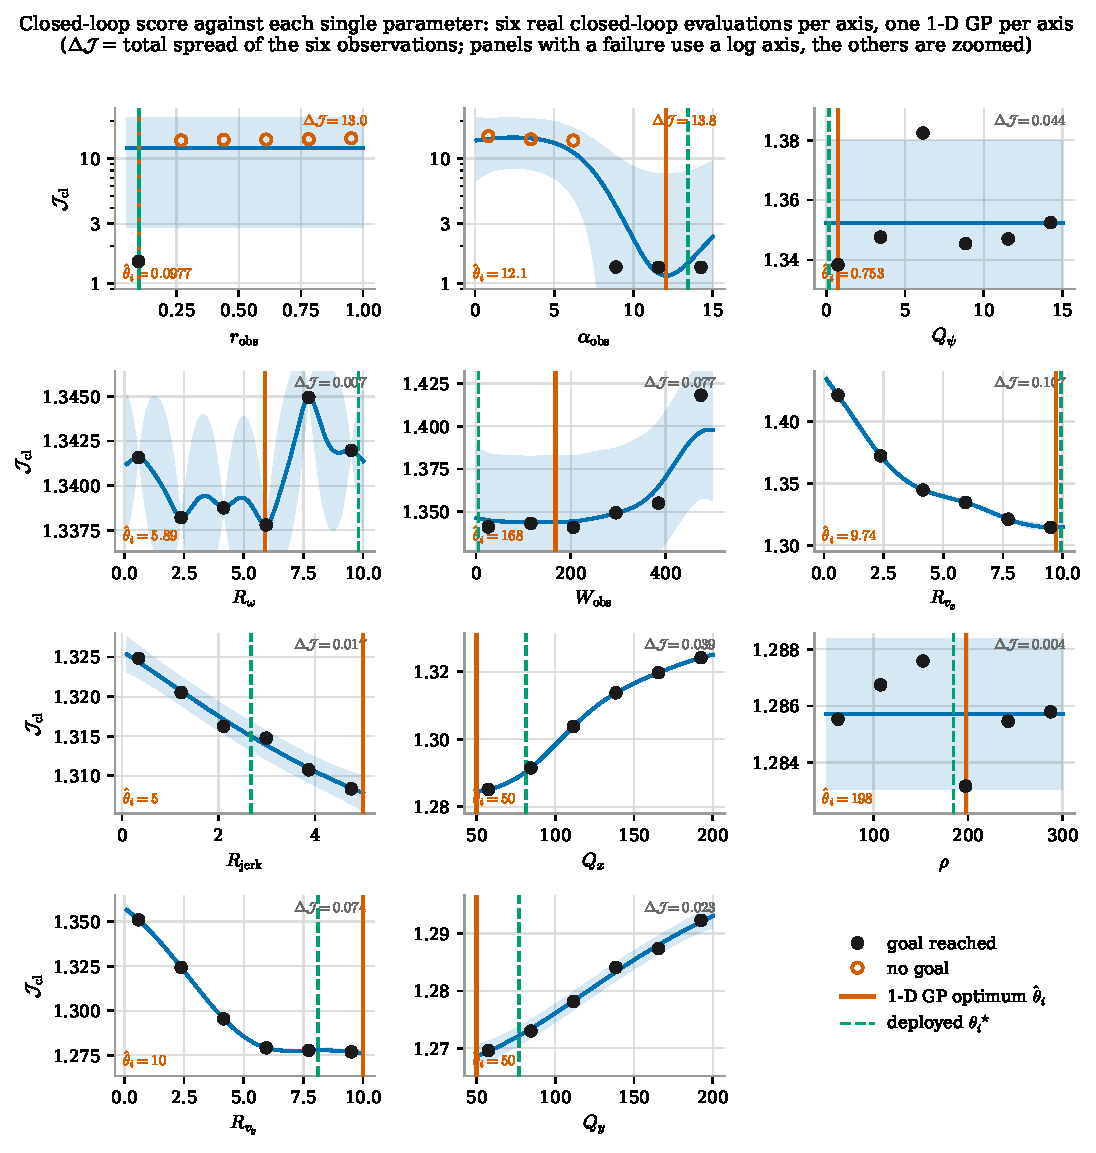
\includegraphics[width=\textwidth]{fig_ofat_curves.pdf}
  \caption{Closed-loop score against each single parameter: six real evaluations per axis with a $1$-D GP
  fitted to each (band: $95\%$ credible interval). Solid vertical line: the GP optimum $\hat\theta_i$; dashed:
  the value shipped in the deployed configuration. $\Delta\mathcal{J}$ is the spread of the six observations
  on that axis; panels containing a failure use a logarithmic axis, the others are zoomed to their own range.
  Axes are swept in the order shown, each optimum being fixed before the next axis is visited.}
  \label{fig:ofatcurves}
\end{figure}

The figure answers, in one page, the question the whole tuning exercise exists to answer.

\emph{Two parameters carry the outcome.} The safety radius $\robs$ and the steepness $\aobs$ each show a
cliff of $\Delta\mathcal{J}\approx13$: on the $\robs$ axis only the smallest of the six sampled values reaches
the goal at all, and on the $\aobs$ axis only three of six do, all of them at $\aobs\gtrsim9$. Every other
axis is flat, with $\Delta\mathcal{J}$ between $0.004$ and $0.107$ --- a factor of at least $130$ smaller.
This is the same conclusion the closed-loop ablation of Section~\ref{sec:sensitivity} reaches by an
independent route, and it is here obtained directly, without a surrogate over eleven coordinates to trust.

\emph{Six evaluations per axis are enough where it matters.} The $\robs$ sweep places its optimum at
$0.0977$~m; the full tuning campaign had converged to $0.098$~m. The $\aobs$ sweep
gives $12.1$~m$^{-1}$ against a deployed $13.4$, and $R_{v_x}$ gives $9.74$ against $9.95$. On the parameters
that move the objective, sixty-six evaluations reproduce a configuration that took an order of magnitude more.

\emph{Five axes terminate on a box bound.} $Q_x$ and $Q_y$ settle at their lower bound of $50$, $R_{v_y}$ and
$\Rjerk$ at their upper bounds, and $\robs$ within $5\%$ of its lower bound. When the optimum of a coordinate
sits on the edge of its admissible interval, the binding constraint is the interval, not the optimizer: the
search ranges of Table~\ref{tab:params} are themselves a design choice that deserves revisiting. For
$\robs$ that revisiting has a physical answer: a safety radius smaller than the robot's half-width is not a
tuning optimum but a modelling hole --- the point-mass plant cannot feel its own body --- and the interval's
lower bound should have been the body radius from the start (Section~\ref{sec:memoryfix}).

\emph{The method fails visibly, not silently.} On $R_\omega$ ($\Delta\mathcal{J}=0.007$) and on $\rho$
($\Delta\mathcal{J}=0.004$) the one-dimensional GP interpolates differences that are of the order of the
run-to-run scatter, and returns a confident-looking optimum which is meaningless. A per-axis scheme therefore
needs the significance floor of Section~\ref{sec:bo}: accept $\hat\theta_i$ only when the axis moves the
objective by more than the noise, and otherwise leave the weight at its default. Applying that rule here
retains $\robs$, $\aobs$, $R_{v_x}$, $R_{v_y}$ and $\Wobs$, and discards the remaining six.

\paragraph{Order matters more than the surrogate.} The same sweeps were also run in the naive arrangement, in
which every axis is swept about one common base point and the eleven per-axis optima are assembled only at the
end. At an identical budget and with identical grids that arrangement returns
$\mathcal{J}_{\mathrm{cl}}=1.354$ against $1.262$ for the sequential scheme, and the evaluation counts explain
why: the common base point --- the midpoint of every interval, $\robs=0.525$~m and $\Wobs=250$ --- is itself a
deadlocked configuration, so ten of the eleven sweeps contain \emph{no} evaluation that reaches the goal.
Those ten curves measure differences between flavours of failure, with spreads of $0.005$ to $0.26$, and their
optima are noise; only the $\robs$ sweep escapes, because that axis alone can undo the deadlock. In the
sequential scheme $\robs$ and $\aobs$ are fixed first, and each of the nine remaining sweeps then runs $6/6$
inside the feasible regime where the objective actually resolves navigation quality. The lesson is not about
Gaussian processes: a one-factor-at-a-time study is only as informative as the operating point it is conducted
around, which is why the axes must be visited in order of influence and each result carried forward.

\begin{table}[htbp]
  \centering
  \small
  \caption{The two per-axis arrangements on the closed-loop objective~\eqref{eq:Jcl} in $\mathrm{E}_c$,
  at an identical budget of $67$ evaluations.}
  \label{tab:ofat}
  \setlength{\tabcolsep}{5.5pt}
  \begin{tabular}{lccccc}
    \toprule
    arrangement & evals & best $\mathcal{J}_{\mathrm{cl}}$ & TTG [s] & $\overline{\|\Delta u\|}$ & $d_{\min}$ [m] \\
    \midrule
    sequential (each optimum fixed before the next sweep) & $67$ & $\mathbf{1.262}$ & $27.9$ & $\mathbf{0.136}$ & $0.69$ \\
    naive (all sweeps about a common base, then assembled) & $67$ & $1.354$ & $27.7$ & $0.286$ & $0.69$ \\
    \bottomrule
  \end{tabular}
\end{table}

\subsection{Trajectory comparison}
\label{sec:trajcompare}

Fig.~\ref{fig:traj1dgp} closes the loop on what the tuning actually buys, comparing the hand-tuned $\thn$
with the per-axis result $\hat\theta$ in both test worlds; the configuration currently shipped in the
repository is drawn dashed as a reference.

\begin{figure}[htbp]
  \centering
  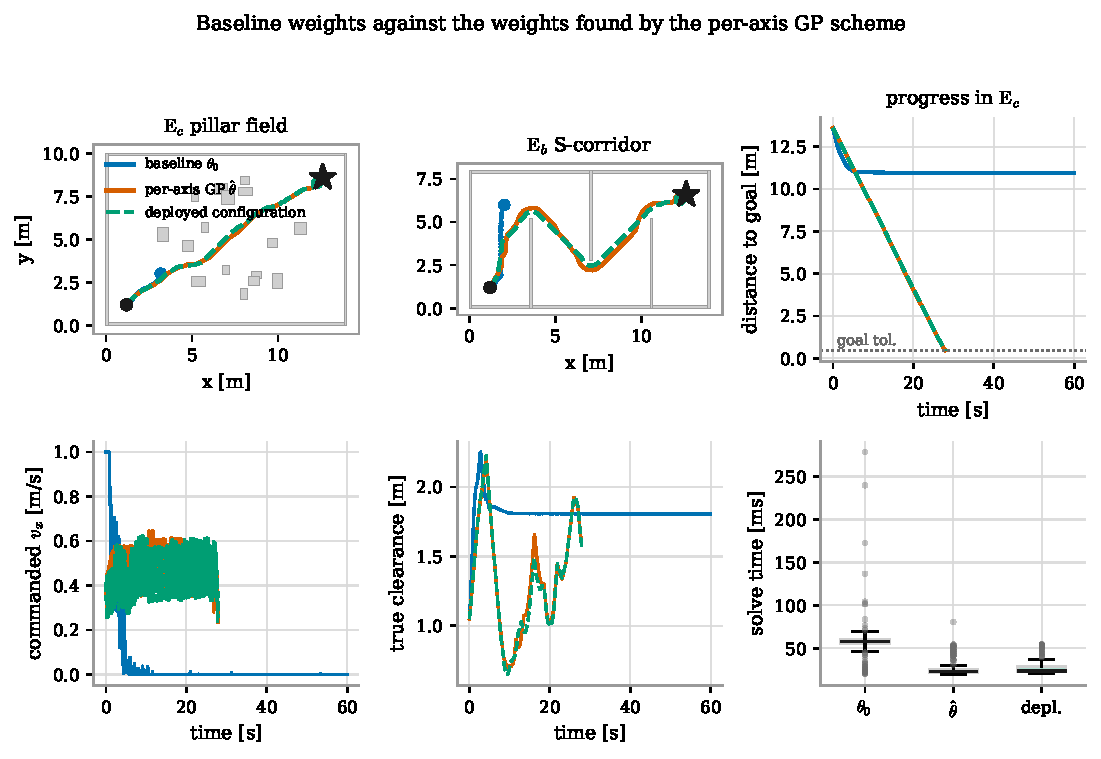
\includegraphics[width=\textwidth]{fig_traj_1dgp.pdf}
  \caption{Executed trajectories under the baseline weights and under the weights found by the per-axis GP
  scheme; the deployed configuration is shown dashed for reference. Top: paths in both worlds and distance to
  goal against time in $\mathrm{E}_c$. Bottom: commanded forward velocity, true clearance, and the
  distribution of per-cycle solve times.}
  \label{fig:traj1dgp}
\end{figure}

The mechanism is unmistakable in the bottom-left panel: under $\thn$ the commanded forward velocity collapses
to zero after ${\sim}10$~s and never recovers, and the distance to goal freezes at $11$~m for the remaining
$50$~s --- the barrier deadlock of Section~\ref{sec:closedloop} in the time domain. The \astar{} layer keeps
producing a valid path throughout; it is the tracker that refuses to follow it. Under $\hat\theta$ the robot
cruises at $0.4$--$0.6$~m/s and reaches the goal in $27.9$~s in $\mathrm{E}_c$ and $36.3$~s in
$\mathrm{E}_b$, while the mean solve time halves and the heavy upper tail of the baseline disappears.
Against the deployed reference the per-axis configuration is marginally slower in the corridor
($36.3$~s against $33.9$~s) and buys with it a minimum clearance of $0.56$~m against $0.30$~m --- nearly twice
the margin, which for a legged platform on a real floor is the better side of that trade.

Animated versions of this comparison, with live readouts of every quantity quoted above, accompany the report
as \texttt{Videos/compare\_pillar\_field.mp4} and \texttt{Videos/compare\_s\_corridor.mp4}.

\subsection{Which weights matter: sensitivity and ablation}
\label{sec:sensitivity}

The per-axis curves of Fig.~\ref{fig:ofatcurves} already contain a sensitivity ranking, and a direct one:
the spread $\Delta\mathcal{J}_i$ of the six observations on each axis measures, in the units of the objective
itself, how much that weight can change the outcome. Table~\ref{tab:params} lists it. Two weights dominate by
three orders of magnitude --- $\Delta\mathcal{J}=13.8$ for $\aobs$ and $13.0$ for $\robs$ --- followed by
$R_{v_x}$ ($0.107$), $\Wobs$ ($0.077$) and $R_{v_y}$ ($0.074$); the remaining six lie between $0.004$ and
$0.044$, at or below the run-to-run scatter.

Two cautions apply to that ranking, and the ablation below settles both. It is measured along axis-aligned
lines, so a weight acting mainly through an interaction is under-ranked --- $\Wobs$ is exactly such a case,
as Section~\ref{sec:barriersweep} shows. And it is measured about a single operating point, so it is a local
statement. A ranking of individual coordinates is therefore validated here by a closed-loop experiment on
weight \emph{groups}, which is insensitive to both objections: the ablation of Fig.~\ref{fig:ablation} and Table~\ref{tab:ablation} does: starting from $\thn$, one group of
weights at a time is replaced by its tuned value.

\begin{table}[htbp]
  \centering
  \small
  \caption{Parameter-group ablation ($90$~s cap). ``$+$ tracking $Q$'' sets $Q_x,Q_y,Q_\psi,\rho$ to their
  tuned values, ``$+$ effort $R$'' sets $R_{v_x},R_{v_y},R_\omega,\Rjerk$, ``$+$ barrier'' sets
  $\Wobs,\aobs,\robs$; each row is otherwise the baseline.}
  \label{tab:ablation}
  \begin{tabular}{llccrrrrr}
    \toprule
    World & group & goal & TTG [s] & dist.\ [m] & $\bar t$ [ms] & $\bar\nu$ & $d_{\min}$ [m] & $\overline{\|\Delta u\|}$ \\
    \midrule
    \multirow{5}{*}{$\mathrm{E}_b$ corridor}
      & baseline $\thn$      & no  & $>90$  & $7.37$  & $39.5$ & $11.8$ & $1.05$ & $0.143$ \\
      & $+$ tracking $Q$     & no  & $>90$  & $6.98$  & $44.3$ & $12.9$ & $1.05$ & $0.128$ \\
      & $+$ effort $R$       & no  & $>90$  & $6.21$  & $40.3$ & $11.7$ & $1.05$ & $0.049$ \\
      & $+$ barrier          & \textbf{yes} & $34.7$ & $17.14$ & $27.3$ & $6.7$  & $0.39$ & $0.272$ \\
      & all ($\thst$)        & \textbf{yes} & $\mathbf{33.9}$ & $16.74$ & $28.4$ & $7.7$  & $0.30$ & $0.166$ \\
    \midrule
    \multirow{5}{*}{$\mathrm{E}_c$ clutter}
      & baseline $\thn$      & no  & $>90$  & $5.88$  & $52.4$ & $16.4$ & $1.05$ & $0.128$ \\
      & $+$ tracking $Q$     & no  & $>90$  & $6.02$  & $66.5$ & $18.2$ & $1.05$ & $0.132$ \\
      & $+$ effort $R$       & no  & $>90$  & $4.28$  & $41.1$ & $12.7$ & $1.05$ & $0.049$ \\
      & $+$ barrier          & \textbf{yes} & $27.8$ & $13.67$ & $28.3$ & $6.9$  & $0.63$ & $0.273$ \\
      & all ($\thst$)        & \textbf{yes} & $\mathbf{27.9}$ & $13.55$ & $26.4$ & $6.9$  & $0.65$ & $0.173$ \\
    \bottomrule
  \end{tabular}
\end{table}

\begin{figure}[htbp]
  \centering
  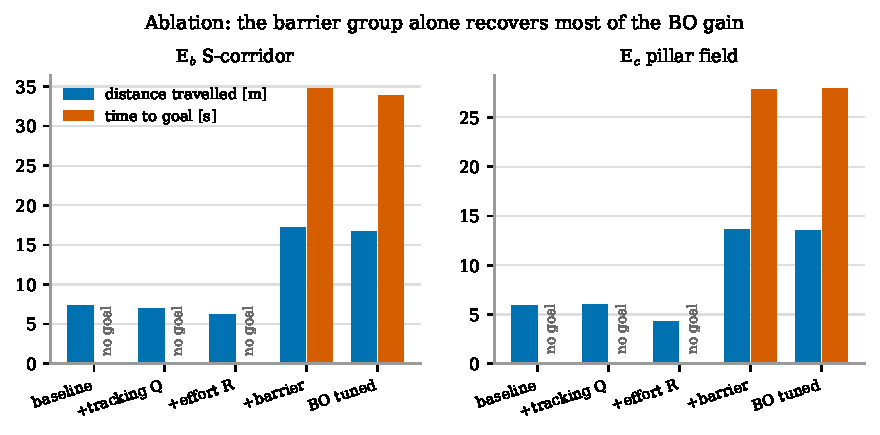
\includegraphics[width=0.92\textwidth]{fig_ablation.pdf}
  \caption{Ablation of the three weight groups in $\mathrm{E}_b$ and $\mathrm{E}_c$. Only the barrier group
  converts a failing controller into a successful one; the effort group then recovers smoothness.}
  \label{fig:ablation}
\end{figure}

The agreement with the surrogate is complete and it is worth stating precisely:
\begin{itemize}
  \item the \textbf{barrier group alone} recovers the entire feasibility gain --- goal reached in $34.7$~s
        against $33.9$~s for the full $\thst$ --- confirming that the dominance of the barrier group measured by the
        per-axis sweeps is not an artefact of the operating point they were measured about;
  \item the \textbf{effort group alone} changes nothing about the outcome but reduces the input increment by
        $62\%$ ($0.128\to0.049$); combined with the barrier group it brings
        $\overline{\|\Delta u\|}$ from $0.272$ down to $0.166$, a $39\%$ smoothing at no cost in time to
        goal. This is exactly the role a control-effort penalty should play: it shapes \emph{how} the task is
        executed, not \emph{whether};
  \item the \textbf{tracking group alone} is actively harmful to the numerics: in $\mathrm{E}_c$ it raises
        the mean solve time from $52.4$ to $66.5$~ms and the iteration count from $16.4$ to $18.2$, because a
        larger $Q$ against an unchanged $\Wobs=500$ sharpens the conflict between two already-large terms.
\end{itemize}
The practical lesson generalises beyond this stack: in a penalty-based MPC, the parameters that decide
success are those of the penalty, and tuning effort is best spent on the relative scaling between the penalty
and the tracking cost rather than on the tracking weights themselves.

\subsection{Prediction horizon and real-time feasibility}
\label{sec:horizon}

Fig.~\ref{fig:horizon} and Table~\ref{tab:horizon} sweep $N\in\{5,10,20,30,50,70\}$ at fixed
$\Delta t=0.1$~s.

\begin{table}[htbp]
  \centering
  \small
  \caption{Prediction-horizon sweep in $\mathrm{E}_b$ (corridor) and $\mathrm{E}_c$ (clutter). $t_{\mathrm{first}}$
  is the cold, first-cycle solve including NLP construction. All configurations reached the goal.}
  \label{tab:horizon}
  \begin{tabular}{rrrrrrrrr}
    \toprule
    & \multicolumn{6}{c}{$\mathrm{E}_b$ corridor} & \multicolumn{2}{c}{$\mathrm{E}_c$ clutter}\\
    \cmidrule(lr){2-7}\cmidrule(lr){8-9}
    $N$ & $\bar t$ [ms] & $t_{95}$ [ms] & $t_{\mathrm{first}}$ [ms] & $\bar\nu$ & TTG [s] & $e_{\mathrm{rms}}$ [m]
    & $\bar t$ [ms] & TTG [s] \\
    \midrule
    $5$  & $7.4$  & $11.0$ & $352$ & $6.2$ & $32.8$ & $0.0438$ & $7.8$  & $26.2$ \\
    $10$ & $9.1$  & $12.9$ & $156$ & $5.9$ & $33.6$ & $0.0456$ & $8.6$  & $27.5$ \\
    $20$ & $13.1$ & $19.4$ & $254$ & $6.4$ & $34.9$ & $0.0472$ & $12.6$ & $27.9$ \\
    $30$ & $17.2$ & $27.5$ & $402$ & $6.5$ & $35.0$ & $0.0472$ & $17.2$ & $27.9$ \\
    $50$ & $27.6$ & $47.0$ & $624$ & $7.7$ & $33.9$ & $0.0463$ & $27.9$ & $27.9$ \\
    $70$ & $41.5$ & $65.3$ & $982$ & $9.1$ & $33.9$ & $0.0471$ & $40.0$ & $27.9$ \\
    \bottomrule
  \end{tabular}
\end{table}

\begin{figure}[htbp]
  \centering
  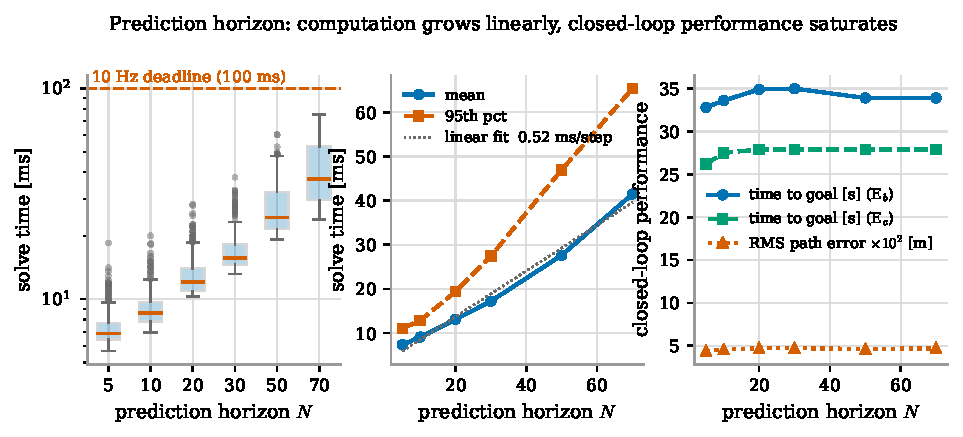
\includegraphics[width=\textwidth]{fig_horizon.pdf}
  \caption{Prediction horizon. Left: distribution of per-cycle solve time (log scale) against the $100$~ms
  deadline. Centre: mean and $95$th percentile with a linear fit of $0.52$~ms per horizon step. Right:
  closed-loop performance --- time to goal in both worlds and RMS path error --- which saturates by
  $N\approx20$.}
  \label{fig:horizon}
\end{figure}

The computational cost is \emph{linear} in $N$: the least-squares fit gives $0.518$~ms per step in
$\mathrm{E}_b$ and $0.503$~ms/step in $\mathrm{E}_c$, with intercepts of $3.4$ and $3.5$~ms. This is the
expected behaviour of a sparse, banded interior-point solve, and it confirms that neither the iteration count
nor the linear algebra degrades with horizon length: $\bar\nu$ grows only from $6.2$ to $9.1$ over a
$14\times$ increase in problem size.

The closed-loop return, on the other hand, saturates. Beyond $N=20$ ($2$~s of preview) the time to goal is
constant to within the $0.1$~s sampling resolution in both worlds, and the RMS path error moves by less than
$4$~mm. The deployed $N=50$ therefore buys nothing measurable over $N=20$ while costing $2.2\times$ the
computation. The reason is structural: the reference~\eqref{eq:ref} only extends $v_{\mathrm{ref}}N\Delta t$
along a path that is itself replanned every second inside a $10$~m window, so preview beyond a couple of
seconds is predicting a reference that no longer exists. This is the single most actionable result of the
study: on the Jetson, where the same solve costs $3$--$4\times$ more, moving from $N=50$ to $N=20$ converts a
$90$--$110$~ms cycle into a comfortable $40$--$50$~ms one at no loss of navigation quality.

Fig.~\ref{fig:solveprofile} confirms that the deadline is respected cycle by cycle and not only on average.
The only violation of the $100$~ms budget in the entire campaign is the first solve, which includes the
symbolic construction of the NLP ($0.35$--$1.0$~s, growing with $N$); from the second cycle onwards the
trace is flat and the tail is bounded by $t_{95}$.

\begin{figure}[htbp]
  \centering
  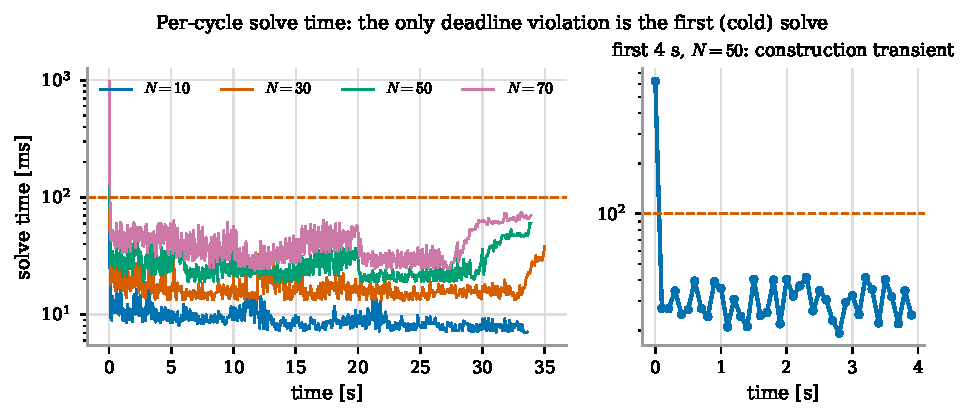
\includegraphics[width=\textwidth]{fig_solve_profile.pdf}
  \caption{Per-cycle solve time (log scale) for four horizons over a full run, and a zoom on the first $4$~s
  at $N=50$. The only deadline violation is the cold first solve, which pays the one-off NLP construction.}
  \label{fig:solveprofile}
\end{figure}

\subsection{Warm start}
\label{sec:warmstart}

Table~\ref{tab:warm} and Fig.~\ref{fig:warmstart} isolate the shift-and-append warm start~\eqref{eq:warm} by
running the same corridor mission with the initial guess replaced by the reference trajectory and zero inputs.

\begin{table}[htbp]
  \centering
  \small
  \caption{Warm start versus cold start, $\mathrm{E}_b$, $N=50$.}
  \label{tab:warm}
  \begin{tabular}{lrrrr}
    \toprule
    & $\bar t$ [ms] & $\bar\nu$ & TTG [s] & distance [m] \\
    \midrule
    shift-and-append warm start & $26.8$ & $7.69$  & $33.9$ & $16.739$ \\
    cold start every cycle      & $43.6$ & $10.93$ & $33.9$ & $16.739$ \\
    \midrule
    change                      & $-38.7\%$ & $-29.6\%$ & $0$ & $<10^{-4}$ \\
    \bottomrule
  \end{tabular}
\end{table}

\begin{figure}[htbp]
  \centering
  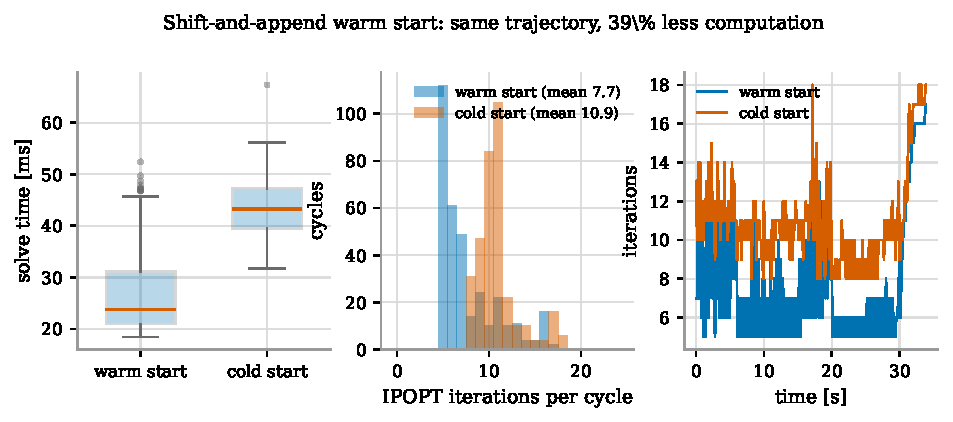
\includegraphics[width=\textwidth]{fig_warmstart.pdf}
  \caption{Warm start: solve-time distribution (left), IPOPT iteration histogram (centre) and iteration count
  over time (right). The executed trajectory is identical to within $10^{-4}$~m; only the computation
  changes.}
  \label{fig:warmstart}
\end{figure}

The two trajectories are identical to $10^{-4}$~m --- the warm start changes \emph{how fast} the same
solution is found, not which solution --- while the computation drops by $38.7\%$ and the iteration count by
$29.6\%$. The histogram shows the mechanism: the cold-start distribution is shifted by roughly three
iterations, with a heavier tail, whereas the warm-started run concentrates at $7$--$8$ iterations. The saving
is real but modest compared with what an active-set or real-time-iteration scheme obtains from a warm start,
for the reason given in Section~\ref{sec:solver}: an interior-point method must re-inflate its barrier
parameter and push the iterate strictly inside the bounds, discarding part of the inherited information.

\subsection{Sampling time and duty cycle}
\label{sec:dtsweep}

A shorter sampling time improves both the discretization fidelity of~\eqref{eq:posedisc} and the resolution at
which the barrier is enforced, but at fixed look-ahead it also increases $N$. Table~\ref{tab:dt} and
Fig.~\ref{fig:dt} sweep $\Delta t$ with the $5$~s window held constant.

\begin{table}[htbp]
  \centering
  \small
  \caption{Sampling-time sweep at fixed $5$~s look-ahead, $\mathrm{E}_b$. The duty cycle is
  $\bar t/\Delta t$: values approaching $100\%$ leave no CPU for the rest of the stack.}
  \label{tab:dt}
  \begin{tabular}{rrrrrr}
    \toprule
    $\Delta t$ [s] & $N$ & $\bar t$ [ms] & duty cycle [\%] & TTG [s] & $e_{\mathrm{rms}}$ [m] \\
    \midrule
    $0.05$ & $100$ & $47.7$ & $95.4$ & $35.95$ & $0.0474$ \\
    $0.10$ & $50$  & $26.9$ & $26.9$ & $33.90$ & $0.0463$ \\
    $0.20$ & $25$  & $17.2$ & $8.6$  & $34.00$ & $0.0483$ \\
    $0.40$ & $13$  & $11.1$ & $2.8$  & $36.40$ & $0.0361$ \\
    \bottomrule
  \end{tabular}
\end{table}

\begin{figure}[htbp]
  \centering
  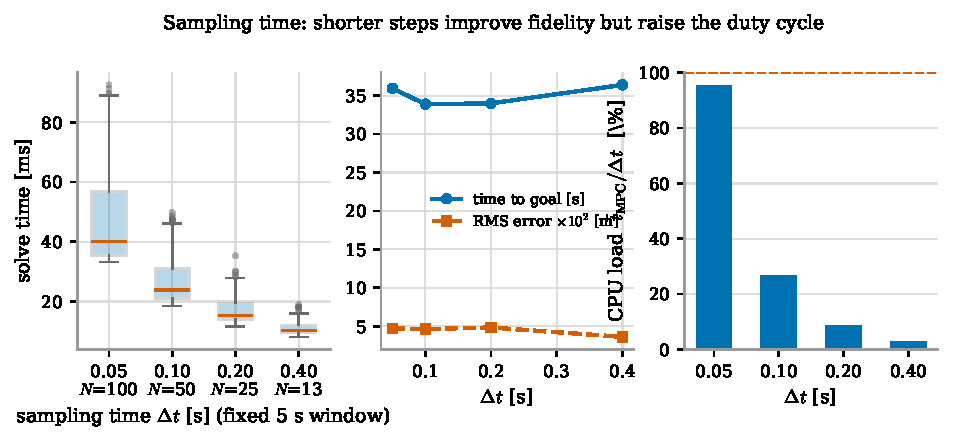
\includegraphics[width=\textwidth]{fig_dt.pdf}
  \caption{Sampling time at fixed look-ahead: solve-time distribution (left), closed-loop performance
  (centre) and duty cycle $\bar t/\Delta t$ against the real-time limit (right).}
  \label{fig:dt}
\end{figure}

The closed-loop metrics are remarkably insensitive --- time to goal varies by $7\%$ and the RMS path error by
$3$~cm over an eight-fold change in $\Delta t$ --- while the duty cycle varies by a factor $34$. At
$\Delta t=0.05$~s the controller consumes $95.4\%$ of its own period on the development machine and is
therefore not deployable at all; $\Delta t=0.1$~s leaves a $3.7\times$ margin, which on a $3$--$4\times$
slower onboard computer is exactly the margin that disappears. The apparent improvement of
$e_{\mathrm{rms}}$ at $\Delta t=0.4$~s is an artefact of coarser sampling of the same error signal, not better
tracking; the corresponding time to goal is the worst of the four, and the barrier is then enforced only
every $0.4$~s, i.e.\ every $20$~cm of travel, which is the inter-sample safety hole discussed in
Section~\ref{sec:barrier}. The deployed $\Delta t=0.1$~s is the correct compromise.

\subsection{Barrier shaping}
\label{sec:barriersweep}

The barrier has three knobs, and Fig.~\ref{fig:barriersweeps} together with Table~\ref{tab:barrier} shows
that two of them govern qualitatively different failure modes.

\begin{table}[htbp]
  \centering
  \small
  \caption{Barrier sweeps. Left block: steepness $\aobs$ in $\mathrm{E}_b$ with $\Wobs=50$,
  $\robs=0.35$~m. Right block: height $\Wobs$ in $\mathrm{E}_c$ with $\aobs=8$, $\robs=0.45$~m.}
  \label{tab:barrier}
  \begin{tabular}{rccrrr@{\hskip 2.2em}rccrr}
    \toprule
    $\aobs$ & goal & TTG [s] & dist.\ [m] & $d_{\min}$ [m] & $\bar\nu$ &
    $\Wobs$ & goal & TTG [s] & dist.\ [m] & $\bar\nu$ \\
    \midrule
    $2.0$   & no  & $>100$ & $16.09$ & $0.985$ & $11.4$ & $0$    & yes & $27.9$ & $13.55$ & $6.9$ \\
    $5.0$   & yes & $55.4$ & $21.45$ & $0.977$ & $8.4$  & $5$    & yes & $27.7$ & $13.59$ & $6.8$ \\
    $8.0$   & yes & $44.8$ & $19.72$ & $0.814$ & $8.7$  & $50$   & no  & $>100$ & $4.63$  & $11.1$ \\
    $13.44$ & yes & $38.5$ & $18.35$ & $0.644$ & $8.1$  & $200$  & no  & $>100$ & $5.01$  & $11.7$ \\
    $25.0$  & yes & $36.8$ & $18.04$ & $0.516$ & $8.1$  & $500$  & no  & $>100$ & $4.34$  & $12.5$ \\
    $40.0$  & yes & $35.1$ & $17.28$ & $0.455$ & $8.0$  &        &     &        &         &       \\
    \bottomrule
  \end{tabular}
\end{table}

\begin{figure}[htbp]
  \centering
  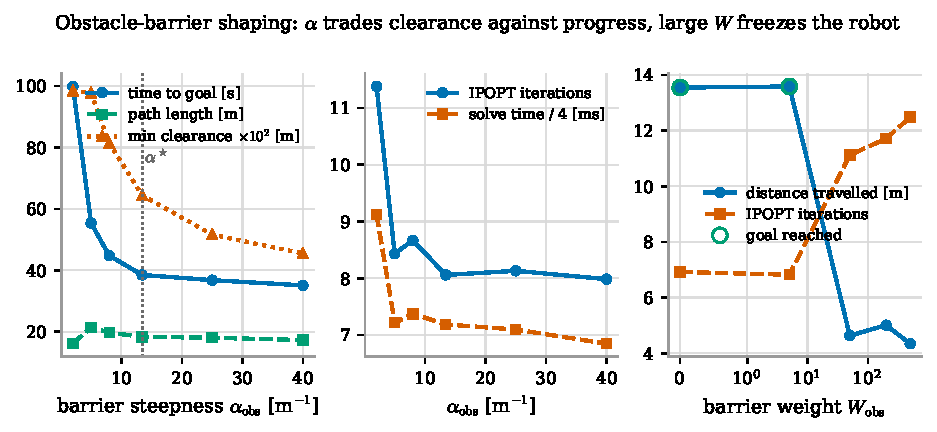
\includegraphics[width=\textwidth]{fig_barrier_sweeps.pdf}
  \caption{Obstacle-barrier shaping. Left: steepness $\aobs$ trades minimum clearance against time to goal
  and path length, with $\thst$'s value marked. Centre: iteration count and solve time against $\aobs$.
  Right: barrier height $\Wobs$ --- above $\Wobs\approx50$ the robot stops making progress (open circles mark
  the runs that reached the goal).}
  \label{fig:barriersweeps}
\end{figure}

\paragraph{Steepness $\aobs$ trades clearance for progress, monotonically.} From $\aobs=5$ to $40$~m$^{-1}$
the time to goal falls from $55.4$ to $35.1$~s and the path shortens from $21.4$ to $17.3$~m, while the
minimum clearance falls from $0.98$ to $0.46$~m: a steep barrier is a \emph{narrow} barrier, so the robot is
allowed to pass closer and takes the shorter route. The interesting end of the sweep is the flat one:
$\aobs=2$~m$^{-1}$ fails to reach the goal at all. A shallow sigmoid is a long-range field --- at
$\aobs=2$ the penalty is still at $27\%$ of its maximum one metre outside $\robs$ --- so every obstacle in the
$3$~m search radius pushes on the whole horizon and the sum of many weak repulsions again produces a stall.
The conditioning cost of steepness predicted in Section~\ref{sec:barrier} is visible but mild in this range
($\bar\nu$ from $8.4$ at $\aobs=5$ to $8.0$ at $\aobs=40$, with the failing $\aobs=2$ run needing $11.4$):
within the tested window, a steeper barrier that engages fewer points is cheaper, not dearer, than a flat one
that engages all of them.

\paragraph{Height $\Wobs$ is a cliff, not a trade-off.} At $\Wobs\in\{0,5\}$ the mission completes in
$27.7$--$27.9$~s; at $\Wobs\ge50$ it never completes, the robot travelling $4.3$--$5.0$~m in $100$~s while
the iteration count rises by $60$--$80\%$ and the solve time by $65$--$120\%$. Two observations follow. First,
this quantitatively reproduces the baseline failure of Section~\ref{sec:closedloop}, which used
$\Wobs=500$ --- the hand-tuned configuration was on the wrong side of the cliff. Second, and more
interesting, $\Wobs=0$ (barrier \emph{off}) also completes the mission with a $0.65$~m minimum clearance:
in a world where \astar{} plans on an inflated grid, the barrier is not what keeps the robot safe on average
--- it is a last-metre guard against the returns that appear between two replanning ticks. The optimizer's
choice of $\Wobs=4.83$ is exactly that reading, and it explains why the tuned configuration is also the
better-conditioned one.

\paragraph{The cliff belongs to the pair $(\Wobs,\robs)$, not to $\Wobs$.} The sweep above holds
$\robs=0.45$~m and $\aobs=8$, and read in isolation it would suggest that a large barrier height is always
fatal. Two configurations found during tuning contradict that: $(\Wobs,\aobs,\robs)=(337,15,0.293)$ and
$(468,12.3,0.053)$ both complete the same mission in $27.7$~s with $\Wobs$ two orders of magnitude above the
``cliff'', and the per-axis optimum of Table~\ref{tab:params} keeps $\Wobs=168$ for the same reason. The controlling quantity is not $\Wobs$ but the barrier
value at the clearance the environment actually permits. Evaluating~\eqref{eq:barrier} per point at
$d=0.65$~m, the clearance the pillar field allows, gives $8.40$ cost units for the failing
$(50,8,0.45)$ setting against $1.59$, $0.30$ and $0.003$ for the two configurations above and for the
deployed vector --- while at $d=0.30$~m the same three configurations rise to $160$, $21$ and $0.30$, i.e.\ they are
steep walls placed close in rather than fields that push from a metre away. A one-dimensional sweep of
$\Wobs$ at fixed $\robs$ therefore measures a slice through an interacting pair, and the height alone is not
the quantity to tune. This also settles the caution raised in Section~\ref{sec:sensitivity}: the small
$\Delta\mathcal{J}=0.077$ measured on the $\Wobs$ axis is not evidence that the barrier height is
unimportant, but a consequence of measuring it along an axis-aligned line at a small $\robs$, where the height
genuinely has little left to do. $\Wobs$ is the clearest example in the study of a weight that a per-axis
scheme under-ranks, and the reason it must be read together with $\robs$ rather than on its own.

\subsection{Effort and rate penalties}
\label{sec:weights}

Fig.~\ref{fig:weights} and Table~\ref{tab:weights} scale the whole effort block, $R\leftarrow\mu R^\star$,
and sweep the rate penalty $\Rjerk$ separately.

\begin{table}[htbp]
  \centering
  \small
  \caption{Left: effort multiplier $\mu$ ($R\leftarrow\mu R^\star$) in $\mathrm{E}_c$. Right: rate penalty
  $\Rjerk$ in $\mathrm{E}_b$. All runs reached the goal.}
  \label{tab:weights}
  \begin{tabular}{rrrr@{\hskip 3em}rrrr}
    \toprule
    $\mu$ & $e_{\mathrm{rms}}$ [m] & $\overline{\|\Delta u\|}$ & TTG [s] &
    $\Rjerk$ & $e_{\mathrm{rms}}$ [m] & $\overline{\|\Delta u\|}$ & TTG [s] \\
    \midrule
    $0.01$ & $0.0452$ & $0.422$ & $27.8$ & $0$     & $0.0471$ & $0.1768$ & $33.9$ \\
    $0.1$  & $0.0447$ & $0.349$ & $27.8$ & $0.2$   & $0.0471$ & $0.1759$ & $33.9$ \\
    $1$    & $0.0473$ & $0.173$ & $27.9$ & $2.68$  & $0.0463$ & $0.1656$ & $33.9$ \\
    $10$   & $0.0620$ & $0.057$ & $28.8$ & $10$    & $0.0475$ & $0.1544$ & $33.9$ \\
    $100$  & $0.0677$ & $0.021$ & $33.9$ & $40$    & $0.0491$ & $0.1407$ & $35.9$ \\
    \bottomrule
  \end{tabular}
\end{table}

\begin{figure}[htbp]
  \centering
  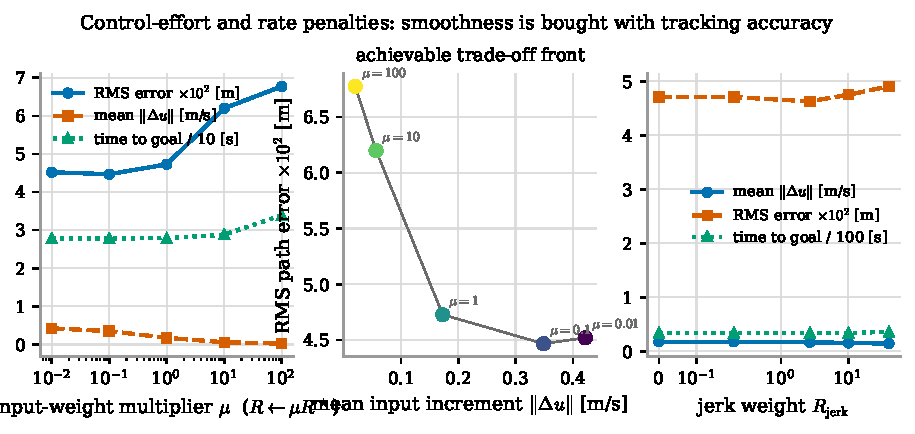
\includegraphics[width=\textwidth]{fig_weights.pdf}
  \caption{Control-effort and rate penalties. Left: metrics against the effort multiplier $\mu$. Centre: the
  achievable trade-off front between input smoothness and tracking accuracy, annotated with $\mu$. Right:
  the rate penalty $\Rjerk$, a comparatively weak knob.}
  \label{fig:weights}
\end{figure}

The effort weight traces a clean Pareto front (centre panel): over four decades of $\mu$ the mean input
increment falls by a factor $20.6$ while the RMS path error grows by $50\%$, and the deployed
$\mu=1$ sits at the knee. The two extremes are both undesirable for a legged platform: at $\mu=0.01$ the
commands chatter ($\overline{\|\Delta u\|}=0.42$~m/s per cycle, i.e.\ nearly the whole velocity range) and at
$\mu=100$ the robot is so reluctant to move that the mission takes $22\%$ longer. Note that this is a
genuinely two-objective problem, and that the scalarisation implicit in~\eqref{eq:cost} --- and in the
tuning objective~\eqref{eq:Jcl}, which prices smoothness at $0.5\,\overline{\|\Delta u\|}$ against time ---
is what selects a single point on that front.

The rate penalty is a much weaker knob: four decades of $\Rjerk$ buy a $20\%$ reduction in
$\overline{\|\Delta u\|}$ and cost $6\%$ in time to goal, with the tracking error essentially unchanged. This
is consistent with the per-axis sweep of Fig.~\ref{fig:ofatcurves}, on which $\Rjerk$ ranks seventh of
eleven with $\Delta\mathcal{J}=0.017$: within this formulation, smoothness is bought far more efficiently
with $R$ than with $\Rjerk$.

\subsection{Cost of the barrier terms}
\label{sec:nobs}

The number of barrier points $M$ enters the NLP linearly ($2M(N+1)$ terms, Table~\ref{tab:nlp}). The measured
cost, Fig.~\ref{fig:nobs}, is
\begin{equation}
  \bar t(M) \;\approx\; 21.8 + 0.237\,M \quad[\mathrm{ms}],
  \label{eq:nobsfit}
\end{equation}
i.e.\ $0.237$~ms per barrier point over the whole solve, or ${\sim}4.6~\mu$s per barrier term per node.
Crucially, the executed trajectory, the iteration count ($6.92$ for every $M$) and the minimum clearance are
unchanged from $M=4$ to $M=30$: in these worlds the twelve nearest returns already describe the local
geometry completely, and additional points only add redundant, inactive terms. $M$ is therefore a pure
computational parameter, and $M=12$ --- the deployed value --- is generous; $M=8$ would save $2$~ms per cycle
with no measurable effect. The maximum solve time, on the other hand, grows sharply with $M$
($0.32$~s at $M=4$ against $1.31$~s at $M=30$), so a large $M$ makes the worst case worse without improving
the average behaviour, which is the wrong trade for a real-time loop.

\begin{figure}[htbp]
  \centering
  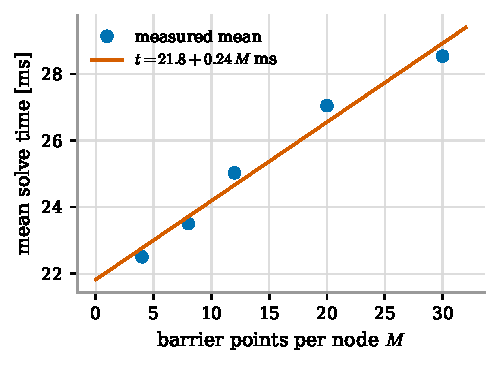
\includegraphics[width=0.5\textwidth]{fig_nobs.pdf}
  \caption{Mean solve time against the number of barrier points per node, with the linear
  fit~\eqref{eq:nobsfit}. The trajectory and the iteration count are identical for all $M$.}
  \label{fig:nobs}
\end{figure}

\subsection{Terminal weight}
\label{sec:terminalsweep}

Fig.~\ref{fig:terminal} and Table~\ref{tab:terminal} sweep $\rho$ over almost three decades.

\begin{table}[htbp]
  \centering
  \small
  \caption{Terminal-multiplier sweep in $\mathrm{E}_b$ ($Q_T=\rho Q$). All runs reached the goal.}
  \label{tab:terminal}
  \begin{tabular}{rrrrrrrr}
    \toprule
    $\rho$ & $1$ & $5$ & $20$ & $50$ & $100$ & $184.78$ & $400$ \\
    \midrule
    TTG [s]                 & $33.9$ & $33.9$ & $33.9$ & $34.0$ & $34.0$ & $33.9$ & $35.1$ \\
    $e_{\mathrm{rms}}$ [m]  & $0.0470$ & $0.0472$ & $0.0473$ & $0.0461$ & $0.0461$ & $0.0463$ & $0.0479$ \\
    $\bar\nu$               & $8.74$ & $8.31$ & $8.13$ & $7.87$ & $7.72$ & $7.69$ & $7.73$ \\
    $\bar t$ [ms]           & $30.7$ & $29.1$ & $28.4$ & $26.9$ & $26.5$ & $27.1$ & $26.7$ \\
    \bottomrule
  \end{tabular}
\end{table}

\begin{figure}[htbp]
  \centering
  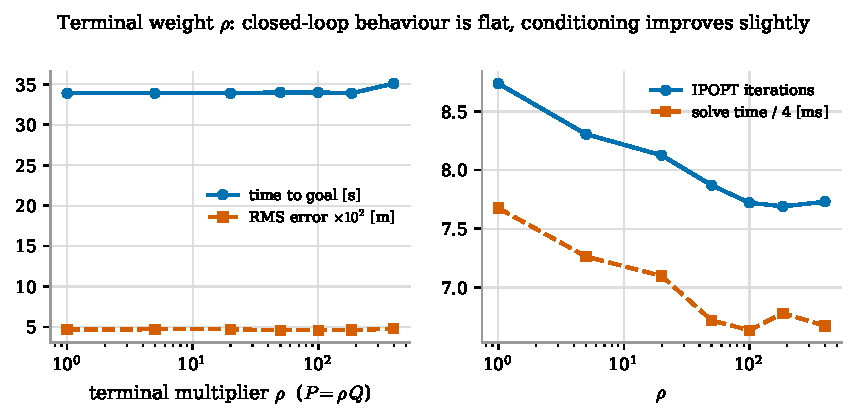
\includegraphics[width=0.9\textwidth]{fig_terminal.pdf}
  \caption{Terminal multiplier $\rho$: closed-loop performance is flat over three decades (left) while the
  conditioning improves slightly (right).}
  \label{fig:terminal}
\end{figure}

Closed-loop behaviour is flat: time to goal changes by $3.5\%$ and only at the extreme $\rho=400$, and the RMS
error by $2$~mm. The one systematic effect is on conditioning --- iterations fall from $8.74$ to $7.69$
($-12\%$) and mean solve time from $30.7$ to $26.5$~ms ($-14\%$) as $\rho$ grows to ${\sim}100$ --- because a
heavier terminal term pins the horizon end-point and removes a soft direction from the search space. This is
the closed-loop counterpart of the analysis in Section~\ref{sec:terminal}: with a $5$~s horizon and a
reference regenerated every second, the terminal cost is a regulariser, not a stabiliser. It also explains why
the Bayesian optimizer assigned $\rho$ the second-lowest sensitivity of all eleven weights
($\tilde\ell_\rho=0.004$): on this problem the terminal weight is genuinely almost free to choose, and the
value $184.78$ it returned should be read as ``anything in $[50,300]$'', not as an optimum.

\subsection{Robustness to model mismatch}
\label{sec:mismatch}

The final campaign perturbs the plant away from the model: the actuator time constants are inflated to
$\tau_v=0.20$~s and $\tau_w=0.16$~s ($+67\%$ and $+60\%$ with respect to the values used by the MPC) and a
constant lateral input disturbance $d_y$ is injected, emulating a gait drift or a lateral slope.

\begin{table}[htbp]
  \centering
  \small
  \caption{Model mismatch, $\mathrm{E}_b$: plant lags $+67\%/+60\%$ larger than the model, plus a constant
  lateral input disturbance $d_y$. ``s.-s.\ offset'' is the mean distance to the \astar{} path over the last
  $10$~s.}
  \label{tab:mismatch}
  \begin{tabular}{rrrr}
    \toprule
    $d_y$ [m/s] & $e_{\mathrm{rms}}$ [m] & s.-s.\ offset [m] & TTG [s] \\
    \midrule
    $0.00$ & $0.0461$ & $0.0368$ & $33.9$ \\
    $0.05$ & $0.0478$ & $0.0376$ & $33.9$ \\
    $0.10$ & $0.0511$ & $0.0445$ & $35.5$ \\
    $0.20$ & $0.0627$ & $0.0602$ & $37.7$ \\
    \bottomrule
  \end{tabular}
\end{table}

\begin{figure}[htbp]
  \centering
  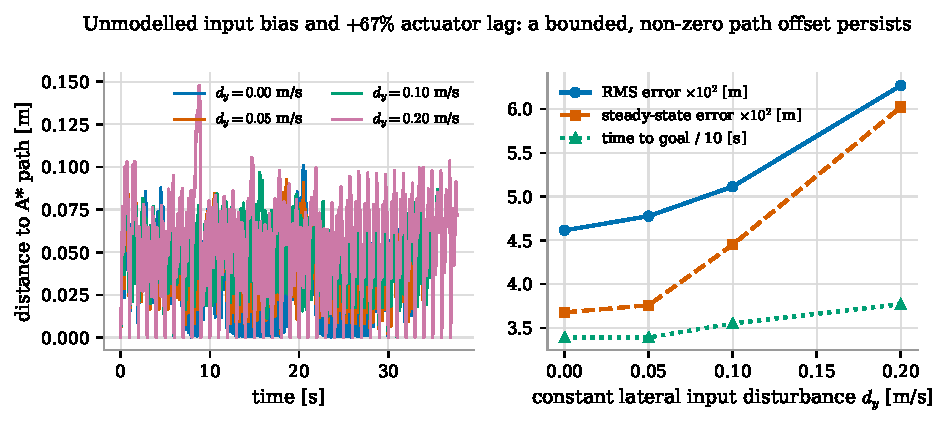
\includegraphics[width=0.92\textwidth]{fig_mismatch.pdf}
  \caption{Model mismatch and input disturbance. Left: distance to the \astar{} path over time for four
  disturbance levels. Right: RMS error, steady-state offset and time to goal against $d_y$. The offset is
  bounded but does not vanish --- the signature of a controller without integral action.}
  \label{fig:mismatch}
\end{figure}

The controller degrades gracefully: a $67\%$ error in the actuator time constant alone (the $d_y=0$ row) costs
essentially nothing, because the mismatch acts on a state the cost does not penalise and the receding horizon
re-corrects at every cycle. The disturbance response, however, exhibits exactly the offset predicted in
Section~\ref{sec:integral}: the steady-state distance to the path grows from $3.7$ to $6.0$~cm and
\emph{does not decay}, while the mission takes $11\%$ longer. The relation is close to linear in $d_y$, as
expected for a proportional-predictive controller against a constant input disturbance: with the tuned
$Q_y=76.8$ and $R_{v_y}=8.1$, the closed-loop lateral stiffness fixes the ratio between offset and
disturbance. Removing the offset requires either augmenting the state with an integrated tracking error or
estimating the disturbance and feeding it forward; neither is present in the deployed formulation, and both
are recommended in Section~\ref{sec:discussion}. It is worth noting that a $6$~cm offset against a path
planned with a $0.30$~m inflation halo is not a safety problem --- it is a performance one.

\subsection{Evidence from the physical robot}
\label{sec:hardware}

The offline harness deliberately isolates the optimization layer; the numbers that matter for deployment come
from the robot. Table~\ref{tab:bags} aggregates the recorded runs of the physical Go2 in three environments,
comparing the hand-tuned baseline with the deployed configuration.

\begin{table}[htbp]
  \centering
  \small
  \caption{Metrics extracted from recorded runs of the physical robot (2--4 runs per world per
  configuration). TTG is the mean over successful runs; solve times are per-cycle statistics of the onboard
  MPC. The run counts are small and several bags are incomplete, so these figures support the solve-time and
  time-to-goal trends but not a success-rate claim.}
  \label{tab:bags}
  \begin{tabular}{llrrrrr}
    \toprule
    World & $\theta$ & TTG [s] & $\bar t$ [ms] & $t_{95}$ [ms] & $t_{\max}$ [ms] & solves \\
    \midrule
    \multirow{2}{*}{indoor office} & $\thn$  & $84.8$  & $46.8$ & $82.6$  & $925$  & $943$ \\
                                   & $\thst$ & $52.3$  & $23.4$ & $40.4$  & $53$   & $746$ \\
    \multirow{2}{*}{open world}    & $\thn$  & $41.6$  & $41.2$ & $59.2$  & $144$  & $1118$ \\
                                   & $\thst$ & $41.9$  & $37.7$ & $76.0$  & $102$  & $816$ \\
    \multirow{2}{*}{warehouse}     & $\thn$  & $474.7$ & $60.5$ & $110.7$ & $1518$ & $2554$ \\
                                   & $\thst$ & $188.5$ & $51.1$ & $100.6$ & $1526$ & $3942$ \\
    \bottomrule
  \end{tabular}
\end{table}

The trend reproduces the simulation result where it should: the harder the environment, the larger the gain.
In the indoor office --- the environment whose recording also provided the replay dataset for the tuning ---
the mean solve time halves ($46.8\to23.4$~ms) and, more importantly, the tail collapses
($t_{\max}$ from $925$ to $53$~ms), which is the difference between a controller that occasionally misses its
deadline and one that does not. In the open world, where the barrier is rarely active, the gain is marginal
($-8.5\%$), exactly as the barrier-dominated sensitivity analysis predicts. The companion
paper \cite{ortolani2026bo}, which evaluates the same two configurations over a larger campaign in Gazebo and
on hardware, reports aggregate reductions of $38.7\%$ in path length, $25.3\%$ in mean solve time and $53.0\%$
in time to goal, with the success rate rising from $65\%$ to $90\%$ in simulation and from $5/10$ to $8/10$
in a real room, and it is the reference for the deployment claim; the contribution of the present report is
the numerical explanation of \emph{why} those gains occur.

Fig.~\ref{fig:trajcmp} shows the effect at the level of a single control cycle, replayed from the recorded
office run: given the same reference and the same LiDAR returns, the tuned weights keep the predicted
trajectory on the path where the baseline is pushed off it by the wide barrier.

\begin{figure}[htbp]
  \centering
  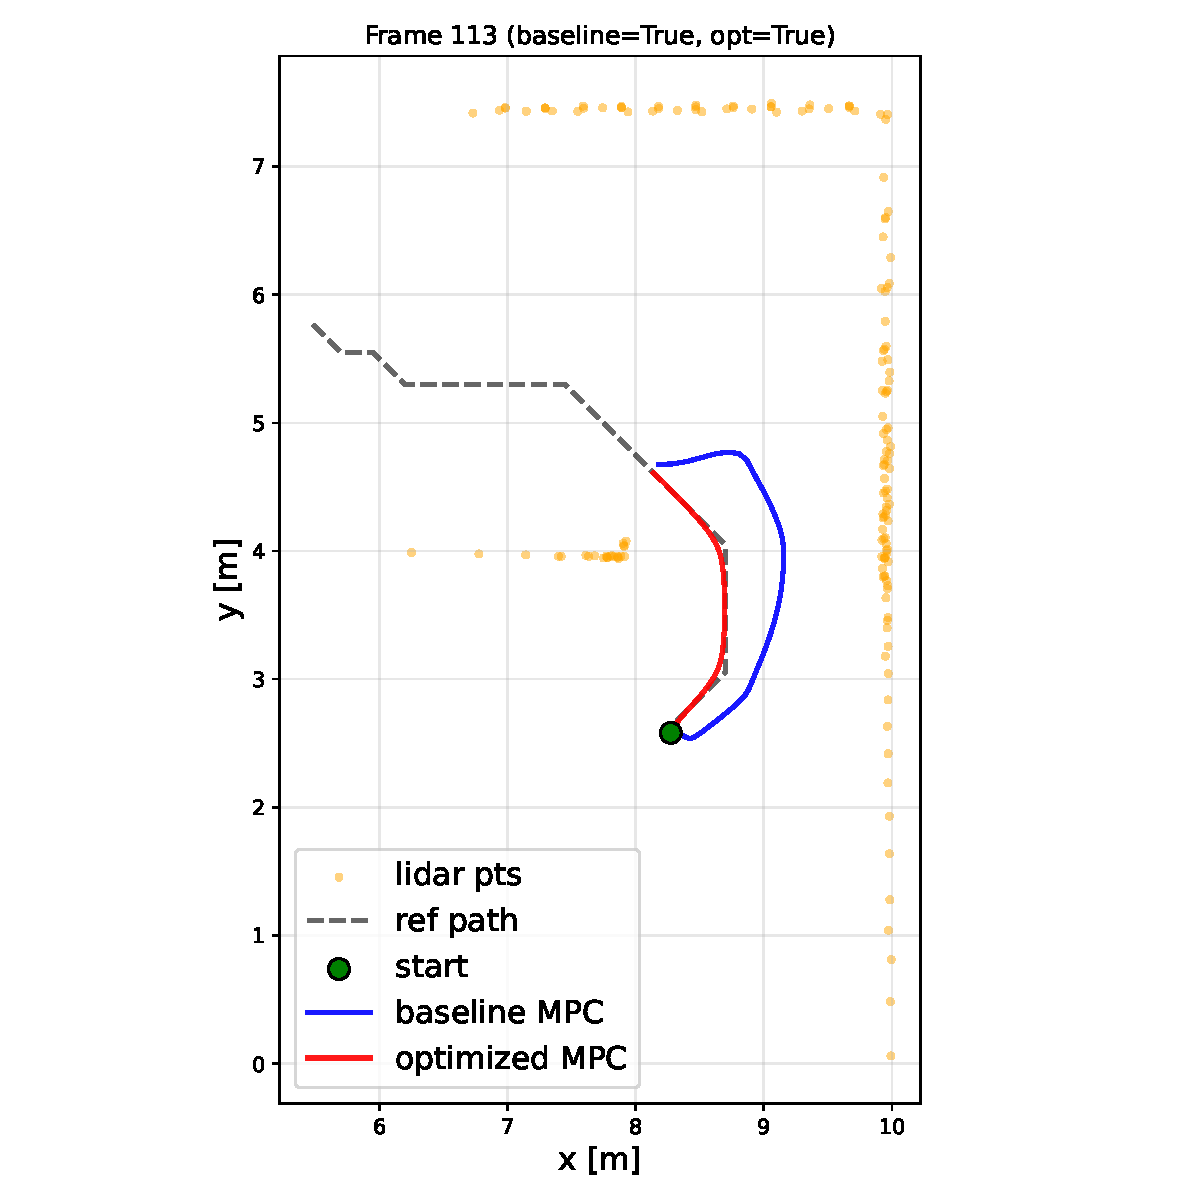
\includegraphics[width=0.52\textwidth]{trajectory_comparison_frame113.pdf}
  \caption{One frame replayed from the recorded office run: \astar{} reference (grey), baseline MPC
  prediction (blue) and tuned prediction (orange) against the LiDAR returns. The tuned controller stays on the
  reference where the baseline is pushed off it by the wide barrier.}
  \label{fig:trajcmp}
\end{figure}

\subsection{Summary of design guidelines}
\label{sec:guidelines}

Table~\ref{tab:guidelines} collects the actionable outcome of the eleven campaigns.

\begin{table}[htbp]
  \centering
  \small
  \caption{Design guidelines extracted from the numerical study.}
  \label{tab:guidelines}
  \begin{tabular}{p{0.20\textwidth}p{0.17\textwidth}p{0.55\textwidth}}
    \toprule
    Parameter & Deployed / suggested & Evidence \\
    \midrule
    Horizon $N$ & $50$ / $\mathbf{20}$ & Cost linear at $0.52$~ms/step; performance saturates at
      $N\!\approx\!20$ in both worlds (\S\ref{sec:horizon}). \\
    Sampling $\Delta t$ & $0.1$~s / keep & $95\%$ duty cycle at $0.05$~s; barrier enforced only every
      $20$~cm at $0.4$~s (\S\ref{sec:dtsweep}). \\
    Barrier height $\Wobs$ & $4.83$ / keep & Cliff at $\Wobs\!\approx\!50$: above it the robot stalls; the
      baseline's $500$ was on the wrong side (\S\ref{sec:barriersweep}). \\
    Steepness $\aobs$ & $13.4$~m$^{-1}$ / keep & Monotone clearance-vs-progress trade-off; flat barriers
      ($\aobs\!\le\!2$) stall and cost more iterations (\S\ref{sec:barriersweep}). \\
    Safety radius $\robs$ & $0.098$ / \textbf{floor at body radius} & The point-mass optimum strips the
      safety net --- a plant with no body cannot price clearance. Floored at $0.30$~m on the platform
      (\S\ref{sec:memoryfix}). \\
    Barrier points $M$ & $12$ / $\mathbf{8}$ & $0.237$~ms per point, identical trajectory and iteration count
      from $M=4$ to $30$; large $M$ inflates the worst case (\S\ref{sec:nobs}). \\
    Effort scaling $R$ & $\mu=1$ / keep & Knee of a $20\times$ smoothness vs $50\%$ accuracy Pareto front
      (\S\ref{sec:weights}). \\
    Rate penalty $\Rjerk$ & $2.68$ / not critical & Weak knob; $20\%$ smoothing over four decades
      (\S\ref{sec:weights}). \\
    Terminal $\rho$ & $184.8$ / not critical & Flat closed loop; mild conditioning gain up to
      $\rho\!\approx\!100$ (\S\ref{sec:terminalsweep}). \\
    Warm start & on / keep & $-38.7\%$ computation at an identical trajectory (\S\ref{sec:warmstart}). \\
    Integral action & absent / \textbf{add} & Persistent $6$~cm offset under a $0.2$~m/s input disturbance
      (\S\ref{sec:mismatch}). \\
    Planner memory & on / \textbf{required} & Without it the rolling-horizon rule livelocks in a two-room
      world (\S\ref{sec:localmin}); with confirmed cells and the re-posed target rule~\eqref{eq:memgoal}
      the same world is solved (\S\ref{sec:memoryfix}). \\
    Weight tuning & per-axis GP, sequential & $67$ rollouts suffice; sweep in order of influence and carry each
      optimum forward --- the naive arrangement leaves $10/11$ curves uninformative (\S\ref{sec:ofat}). \\
    Weights worth tuning & $\robs,\aobs$ (then $R$) & $\Delta\mathcal{J}\approx13$ against $\le0.11$ for the
      other nine; six weights fall below the significance floor (\S\ref{sec:sensitivity}). \\
    \bottomrule
  \end{tabular}
\end{table}

%=============================================================================
\section{Discussion and limitations}
\label{sec:discussion}

\paragraph{What the formulation guarantees, and what it does not.} The NLP is always feasible, because the
only constraints are the dynamics and the input box; this is a real robustness property for a $10$~Hz loop
with no fallback. But there is no terminal set, no terminal constraint and no Lyapunov argument, so nominal
asymptotic stability and recursive feasibility in the sense of
\cite{mayne2000constrained,chen1998quasi} are \emph{not} established, and the analysis of
Section~\ref{sec:terminal} shows that the deployed terminal weight is far from the infinite-horizon
cost-to-go of even the linearised dynamics. Safety is likewise not guaranteed: the clearance constraint is a
finite penalty and it is imposed only at the discrete nodes. A formulation with a discrete-time control
barrier function constraint \cite{ames2019cbf}, or with a soft constraint plus explicitly bounded slack,
would recover a certificate; both make the NLP harder and can render it infeasible precisely when the robot
is already too close to an obstacle, which is why the deployed system prefers the penalty. Quantifying that
trade-off is the most valuable extension of this study.

\paragraph{The weakest link is not the optimizer.} Every campaign in Section~\ref{sec:performance} solved its
NLP successfully --- zero solver failures in more than $20\,000$ solves --- and the one systematic failure of
the whole system is a \emph{modelling} failure: the greedy rolling-horizon target
rule~\eqref{eq:localgoal}, which discards the topology of the free space and, combined with the volatile grid
and the non-negativity of $v_x$, produces the livelock of Section~\ref{sec:localmin}.
Section~\ref{sec:memoryfix} repairs it at the level where it lives: the ray becomes the shortest path on a
confirmed-cell memory, and the repair is validated both in the harness and in a physics simulation of the
same world. What remains open is the cleaner formulation still --- putting the local target inside the
optimization, for instance as a receding-horizon target chosen to minimise a value function computed on the
remembered map, rather than fixing it by a graph search before the NLP is even built.

\paragraph{Limits of the tuning.} The per-axis scheme buys its sample efficiency with an assumption of
additive separability, and that assumption is not exactly true: Section~\ref{sec:barriersweep} exhibits the
$(\Wobs,\robs)$ interaction it cannot represent. Sweeping the dominant coordinate first and carrying each
optimum forward contains the damage, and the assembled vector is verified by evaluation rather than assumed
to be optimal, but a genuine two-parameter interaction can only be found by a joint search over the pair ---
which, restricted to the two or three coordinates the sweeps identify as decisive, would be affordable and is
the natural next step. Two further limits are worth stating. The tuning objective~\eqref{eq:Jcl} was evaluated
in a single world, so the weights are optimal for a pillar field and merely good elsewhere; a weighted sum
over several worlds would cost proportionally more rollouts. And five of the eleven axes terminate on a box
bound (Table~\ref{tab:params}), so the intervals are binding and the reported optima are, on those axes,
statements about the box as much as about the objective.

\paragraph{Scope of the numbers.} All timings were obtained on a laptop-class x86 CPU. The onboard Jetson Orin
Nano is roughly $3$--$4\times$ slower, so the deployed $N=50$, $\Delta t=0.1$~s configuration sits much closer
to its deadline on the robot than Fig.~\ref{fig:horizon} suggests --- which is precisely why the
$N\!\to\!20$ recommendation matters. The plant used in the harness is the MPC's own model perturbed in
Section~\ref{sec:mismatch}; it contains no leg dynamics, no terrain and no LiDAR occlusion, so the absolute
success rates are optimistic while the relative comparisons, which is what the study is about, are not
affected.

%=============================================================================
\section{Conclusions}
\label{sec:conclusions}

This report analysed a deployed map-free navigation stack as what it is numerically: two optimization programs
solved at every cycle --- an exact \astar{} search on a Gaussian occupancy grid and a $456$-variable
nonlinear program with actuator-lag dynamics and a smooth obstacle barrier --- plus one black-box program
solved offline to choose the eleven cost weights of the second.

The main quantitative findings are the following. The problem is genuinely real-time: the interior-point solve
costs $0.52$~ms per horizon step, is linear in $N$, needs $7$--$9$ iterations per cycle, and respects a
$100$~ms budget at every cycle except the first, which pays the one-off symbolic construction. The
shift-and-append warm start removes $38.7\%$ of that cost while reproducing the same trajectory to
$10^{-4}$~m. Closed-loop performance saturates at $N\approx20$, so the deployed $N=50$ costs $2.2\times$ more
computation than the task requires. Tuning the eleven weights with one one-dimensional Gaussian process per
weight --- $67$ closed-loop rollouts in total --- changes the outcome qualitatively rather than
quantitatively: the hand-tuned baseline never reaches the goal in any of the three test worlds, the tuned
configuration does, while also halving the mean solve time and cutting the iteration count by up to $58\%$.
The eleven measured curves and an independent closed-loop ablation identify the same cause: two weights out
of eleven decide the outcome, and the hand-tuned barrier they parametrise was wide enough for its repulsive
field, rather than the tracking cost, to dictate the solution. Sweeping the axes in order of influence and
carrying each optimum forward is what makes so small a budget sufficient --- run naively about a single base
point, the same sweeps leave ten of eleven curves measuring differences between failures.

Two negative results are as informative as the positive ones. First, the deployed heuristic terminal cost is
$40\times$ heavier than the exact infinite-horizon cost-to-go on position, ignores the terminal velocity
states entirely, and the closed loop is nonetheless indifferent to it over three decades --- with a $5$~s
horizon and a reference regenerated every second, the terminal weight regularises but does not stabilise.
Second, and more consequentially, the only systematic failure of the system is not in the optimization at all:
the greedy rolling-horizon target rule livelocks in a two-room world where every individual NLP is solved
correctly. Re-posing that rule on a confirmed-cell memory --- the ray replaced by the shortest path on the
remembered map, of which the ray is the empty-memory special case --- eliminates the livelock structurally:
the same world is then solved in $43$~s and well under half the distance the failing controller wastes,
with the NLP, the weights and the solver untouched. Posing the right problem remains harder than solving it well; it is
also, on this evidence, where the performance was hiding.

The natural continuations follow directly from the analysis: add integral action or a disturbance estimator to
remove the measured steady-state offset; re-run the outer optimization on a widened box and against a
closed-loop, mission-level objective, which the harness built for this report makes affordable; reduce
$N$ to $20$ and $M$ to $8$ to recover the resulting computational headroom on the onboard computer; and fold
the target choice of Section~\ref{sec:memoryfix} into the optimization itself, so that the quality of the
problem being posed matches, everywhere, the quality of the solver answering it.

%=============================================================================
\section*{Reproducibility}
\addcontentsline{toc}{section}{Reproducibility}

Every figure and table in Section~\ref{sec:performance} is generated by an offline harness that imports the
production planner and tracker from the project repository, runs the parametric campaigns in closed loop
(${>}20\,000$ IPOPT solves in total) and serialises the logged signals; the figures are then produced from
those logs. The tuning curves of Fig.~\ref{fig:ofatcurves} come from $67$ additional closed-loop rollouts,
six per axis plus one confirmation of the assembled vector, and the hardware figures from recorded ROS~2 bags
of the physical robot. The deployed parameter vector $\thst$ of Table~\ref{tab:params} is the one shipped in
\texttt{src/a\_star\_mpc\_planner/} \texttt{config/planner\_params.yaml}, with one deliberate exception:
the safety radius is floored at the body radius, $\robs=0.30$~m (Section~\ref{sec:memoryfix}). Animated versions of
Fig.~\ref{fig:traj1dgp}, showing the three configurations running the same mission side by side with live
readouts of every quantity quoted in Section~\ref{sec:trajcompare}, accompany this report as
\texttt{Videos/compare\_pillar\_field.mp4} and \texttt{Videos/compare\_s\_corridor.mp4}. Solve times in those
recordings are wall-clock and therefore load-dependent: their absolute values differ from
Table~\ref{tab:closedloop} by the machine load at recording time, while the ratio between configurations is
stable to within $1\%$. The memory study of Section~\ref{sec:memoryfix} ships with its own artefacts: the
rebuilt harness lives under \texttt{harness/} in the project repository (worlds, closed loop, figure and
video generation), the memory-augmented rule is the production module
\texttt{a\_star\_mpc\_planner/global\_memory\_planner.py} wired into the \astar{} node behind the
\texttt{use\_global\_memory} parameter, the Gazebo replica of $\mathrm{E}_a$ is
\texttt{sim\_worlds/worlds/office\_tworoom.world}, and the animated runs --- harness and Gazebo, memoryless
and memory-augmented --- are \texttt{Videos/Ea\_star\_nomem.mp4}, \texttt{Videos/Ea\_star\_mem.mp4},
\texttt{Videos/Eb\_star\_mem.mp4}, \texttt{Videos/Ec\_star\_mem.mp4},
\texttt{Videos/gazebo\_tworoom\_memoryless.mp4} and \texttt{Videos/gazebo\_tworoom\_memory.mp4}.

%=============================================================================
\bibliography{bibliography}

\end{document}
